\documentclass{article} % For LaTeX2e
\usepackage{iclr2026_conference,times}

% Optional math commands from https://github.com/goodfeli/dlbook_notation.
\input{math_commands.tex}

\usepackage[utf8]{inputenc} % allow utf-8 input
\usepackage[T1]{fontenc}    % use 8-bit T1 fonts
\usepackage{hyperref}       % hyperlinks
\usepackage{url}            % simple URL typesetting
\usepackage{booktabs}       % professional-quality tables
\usepackage{amsfonts}       % blackboard math symbols
\usepackage{nicefrac}       % compact symbols for 1/2, etc.
\usepackage{microtype}      % microtypography
\usepackage{xcolor}         % colors

%% additional packages:
 \usepackage{graphicx}
\usepackage{algorithm}
\usepackage{algpseudocode} 
\usepackage{amsmath}
\usepackage[english]{babel}
\usepackage{subcaption}
\usepackage{multirow}
\usepackage{xspace}
\usepackage{bbm}
\usepackage{cleveref}
\crefformat{equation}{eq.~(#2#1#3)}
\usepackage{wrapfig}
\usepackage{enumitem}
\usepackage{adjustbox}


\newcommand{\mr}[2]{\multirow{#1}{*}{#2}}
\newcommand{\mc}[3]{\multicolumn{#1}{#2}{#3}}

\newcommand{\amazon}{\texttt{rel-amazon}\xspace}
\newcommand{\fone}{\texttt{rel-f1}\xspace}
\newcommand{\event}{\texttt{rel-event}\xspace}
\newcommand{\avito}{\texttt{rel-avito}\xspace}
\newcommand{\stack}{\texttt{rel-stack}\xspace}
\newcommand{\relbench}{\textsc{RelBench}\xspace}
\newcommand{\syntherela}{\textsc{SyntheRela}\xspace}
\newcommand{\salt}{\texttt{rel-salt}\xspace}
\newcommand{\ratebeer}{\texttt{rel-ratebeer}\xspace}
\newcommand{\mimic}{\texttt{rel-mimic}\xspace}
\newcommand{\arxiv}{\texttt{rel-arxiv}\xspace}


\newcommand{\valtimestamp}{\textsc{val\_timestamp}\xspace}
\newcommand{\testtimestamp}{\textsc{test\_timestamp}\xspace}


\newcommand{\itemPlant}{\texttt{item-plant}\xspace}
\newcommand{\itemShippoint}{\texttt{item-shippoint}\xspace}
\newcommand{\itemIncoterms}{\texttt{item-incoterms}\xspace}
\newcommand{\SalesOffice}{\texttt{sales-office}\xspace}
\newcommand{\SalesGroup}{\texttt{sales-group}\xspace}
\newcommand{\SalesPayterms}{\texttt{sales-payterms}\xspace}
\newcommand{\SalesShipcond}{\texttt{sales-shipcond}\xspace}
\newcommand{\SalesIncoterms}{\texttt{sales-incoterms}\xspace}


\newcommand{\resultsPosition}{\texttt{results-position}\xspace}
\newcommand{\qualifyingPosition}{\texttt{qualifying-position}\xspace}
\newcommand{\reviewRating}{\texttt{review-rating}\xspace}

\newcommand{\searchstreamClick}{\texttt{searchstream-click}\xspace}
\newcommand{\searchinfoLoggedon}{\texttt{searchinfo-isuserloggedon}\xspace}
\newcommand{\eventInterested}{\texttt{event\_interest-interested}\xspace}

\newcommand{\badgesClass}{\texttt{badges-class}\xspace}


\title{\relbench v2: A Large-Scale Benchmark and Repository for Relational Data}

% Authors must not appear in the submitted version. They should be hidden
% as long as the \iclrfinalcopy macro remains commented out below.
% Non-anonymous submissions will be rejected without review.

\author{Justin Gu$^1$,
Rishabh Ranjan$^1$,
Charilaos Kanatsoulis$^1$,
Haiming Tang$^2$,
Martin Jurkovic$^3$,\\
\textbf{Valter Hudovernik$^4$,
Mark Znidar$^5$,
Pranshu Chaturvedi$^1$,
Parth Shroff$^1$,
Fengyu Li$^1$,}\\
\textbf{Jure Leskovec$^1$}\\
% \thanks{ Use footnote for providing further information about author (webpage, alternative address)---\emph{not} for acknowledging funding agencies.  Funding acknowledgements go at the end of the paper.} \\
$^1$Stanford University,
$^2$National University of Singapore,
$^3$University of Ljubljana,
$^4$Kumo AI,\\
$^5$University of Oxford\\
\texttt{\{justingu,ranjanr,jure\}@stanford.edu} \\
Website: \textcolor{cyan}{\url{https://relbench.stanford.edu}}
% \And
% Ji Q. Ren \& Yevgeny LeNet \\
% Department of Computational Neuroscience \\
% University of the Witwatersrand \\
% Joburg, South Africa \\
% \texttt{\{robot,net\}@wits.ac.za} \\
% \AND
% Coauthor \\
% Affiliation \\
% Address \\
% \texttt{email}
}

% The \author macro works with any number of authors. There are two commands
% used to separate the names and addresses of multiple authors: \And and \AND.
%
% Using \And between authors leaves it to \LaTeX{} to determine where to break
% the lines. Using \AND forces a linebreak at that point. So, if \LaTeX{}
% puts 3 of 4 authors names on the first line, and the last on the second
% line, try using \AND instead of \And before the third author name.

\newcommand{\fix}{\marginpar{FIX}}
\newcommand{\new}{\marginpar{NEW}}

\iclrfinalcopy % Uncomment for camera-ready version, but NOT for submission.
\begin{document}


\maketitle

\begin{abstract}
Relational deep learning (RDL) has emerged as a powerful paradigm for learning directly on relational databases by modeling entities and their relationships across multiple interconnected tables. As this paradigm evolves toward larger models and relational foundation models, scalable and realistic benchmarks are essential for enabling systematic evaluation and progress. In this paper, we introduce \relbench v2, a major expansion of the \relbench benchmark for RDL. \relbench v2 adds four large-scale relational datasets spanning scholarly publications, enterprise resource planning, consumer platforms, and clinical records, increasing the benchmark to 11 datasets comprising over 22 million rows across 29 tables. We further introduce autocomplete tasks, a new class of predictive objectives that require models to infer missing attribute values directly within relational tables while respecting temporal constraints, expanding beyond traditional forecasting tasks constructed via SQL queries. In addition, \relbench v2 expands beyond its native datasets by integrating external benchmarks and evaluation frameworks: we translate event streams from the Temporal Graph Benchmark into relational schemas for unified relational–temporal evaluation, interface with ReDeLEx to provide uniform access to 70+ real-world databases suitable for pretraining, and incorporate 4DBInfer datasets and tasks to broaden multi-table evaluation coverage. Experimental results demonstrate that RDL models consistently outperform single-table baselines across autocomplete, forecasting, and recommendation tasks, highlighting the importance of modeling relational structure explicitly. 

% In addition, \relbench v2 integrates temporal interaction datasets from the Temporal Graph Benchmark by translating event streams into normalized relational schemas, enabling unified evaluation of relational and temporal learning methods within a common framework. Experimental results demonstrate that RDL models consistently outperform single-table baselines across autocomplete, forecasting, and recommendation tasks, highlighting the importance of modeling relational structure explicitly. 
% \relbench v2 provides a comprehensive benchmark for advancing RDL and enabling the development and evaluation of relational foundation models.
\end{abstract}


\section{Introduction} \label{sec:intro}
Relational databases are the primary storage abstraction for structured data across enterprise, scientific, and healthcare systems. They organize information across multiple tables interconnected via primary–foreign key relationships, capturing rich structural and temporal dependencies between entities. Forecasting tasks such as predicting customer churn, estimating sales, recommending products, and anticipating system or patient outcomes are central to real-world decision making and have driven significant interest in applying machine learning to relational data. 


% However, traditional machine learning pipelines typically rely on manually flattening relational schemas into single tables through feature engineering and aggregation. This process is labor-intensive, requires substantial domain expertise, and often fails to fully exploit the relational structure and multi-table dependencies inherent in the data.

Relational deep learning (RDL) \citep{relbench, rdl} has emerged as a powerful paradigm for learning directly on relational databases, reducing the human effort and engineering complexity of traditional machine learning pipelines that rely on manually flattening relational schemas into single tables through feature engineering and aggregation. Instead, RDL treats relational databases as heterogeneous graphs and applies graph neural networks \citep{relbench,chen2025relgnn} and other relational representation learning architectures \citep{dwivedi2025relational,dwivedi2025relational2} to model entities and their relationships directly. RDL models have demonstrated state-of-the-art performance in forecasting tasks over relational data.

% Relational deep learning (RDL) \cite{relbench}, \cite{rdl} has emerged as a promising paradigm for learning directly on relational databases, shifting away from traditional machine learning pipelines typically rely on manually flattening relational schemas into single tables through feature engineering and aggregation. RDL treats relational schemas as heterogeneous graphs and applying graph neural networks or other relational representation learning architectures. Recent work has demonstrated that relational deep learning models can outperform traditional feature-engineered tabular models across a wide range of predictive tasks while significantly reducing human effort and engineering complexity.

% At the same time, the machine learning landscape has shifted toward foundation models, which are pretrained on large and diverse datasets to learn transferable representations. This paradigm has transformed natural language processing and computer vision, and has recently extended to tabular data, where pretrained models have demonstrated strong performance on forecasting and predictive tasks across datasets \cite{tabpfn,tabpfnv2,tabicl}. These results highlight the potential of large-scale pretraining but only focus on single table data.

% More recently, early efforts have begun to develop foundation models for relational databases~\citep{kumorfm, griffin, ranjan2025relational}, leveraging relational deep learning architectures to learn representations across multiple tables and their interdependencies. Relational databases represent a natural next frontier for foundation models due to their ubiquity, structural complexity, and broad coverage of real-world applications. However, progress in this direction critically depends on the availability of benchmarks and datasets with sufficient scale, diversity, and well-defined training objectives to enable the learning and evaluation of transferable relational representations.

At the same time, the machine learning landscape has shifted toward foundation models, which are pretrained on large and diverse datasets to learn transferable representations. This paradigm has transformed natural language processing and computer vision, and has recently extended to tabular data, where pretrained models achieve strong performance across predictive tasks \citep{tabpfn,tabpfnv2,tabicl}. However, these approaches focus on single-table data and do not capture the multi-table structure of relational databases. To address this limitation, recent efforts~\citep{kumorfm, griffin, ranjan2025relational} develop foundation models for relational databases, leveraging RDL architectures to model entities and their interdependencies across tables. Given their ubiquity and structural richness, relational databases represent a natural next frontier for foundation models, motivating benchmarks that capture realistic relational structure and predictive tasks.

To support machine learning research for forecasting on relational databases, \cite{relbench} introduced  \relbench, the first benchmark for RDL. \relbench v1 provided a collection of real-world relational databases along with forecasting tasks that require predicting future outcomes such as entity churn, sales, or recommendations. These tasks enabled standardized evaluation of relational learning models and demonstrated the effectiveness of RDL compared to traditional approaches.

In this work, we introduce  \relbench v2, a significant expansion of the benchmark that introduces new datasets, new task types, and a new paradigm for relational prediction. \relbench v2 adds four new large-scale relational datasets spanning diverse domains, increasing the total number of datasets to eleven. These include \arxiv, a scholarly publication database capturing papers, authors, categories, and citation relationships; \salt, an enterprise resource planning dataset modeling sales orders and business workflows; \ratebeer, a consumer platform dataset containing user interactions, product information, and reviews; and \mimic, a clinical dataset derived from electronic health records. Together, these datasets introduce new relational structures, domains, and predictive challenges, and collectively contain over 22 million rows across 29 tables. 

In addition to expanding the datasets, \relbench v2 introduces new predictive tasks and extends the benchmark with multiple strategic integrations of diverse external benchmarks and diagnostic frameworks. Most notably, \relbench v2 introduces autocomplete tasks, where the objective is to predict values of existing columns in relational tables at a given timestamp, requiring models to infer missing values from relational and temporal context while preventing information leakage. In addition, as subsequent efforts following \relbench v1 have expanded the scale and diversity of relational benchmarks, we integrate several of these into \relbench v2. These include temporal interaction datasets from the Temporal Graph Benchmark (TGB) \citep{rossi2020temporal}, widespread RDL evaluation on 70+ relational databases via ReDeLEx \citep{peleska2025redelex}, and the 4D design space for graph-centric relational modeling from 4DBInfer \citep{wang20244dbinfer}. Additional discussion on RDL and relational foundation models can be found in Appendix \ref{sec:related-work}.


% In addition to expanding the datasets, \relbench v2 introduces new predictive tasks and extends the benchmark to support temporal interaction datasets from the Temporal Graph Benchmark (TGB) \citep{rossi2020temporal}. Most notably, \relbench v2 introduces autocomplete tasks, where the objective is to predict values of existing columns in relational tables at a given timestamp, requiring models to infer missing values from relational and temporal context while preventing information leakage. \relbench v2 also incorporates TGB datasets by translating temporal interaction streams into normalized relational schemas consisting of entity and event tables with primary–foreign key relationships and timestamp cutoffs. This enables evaluation of RDL models on large-scale temporal interaction data within the same database abstraction and temporal evaluation framework used throughout \relbench. 

% \textbf{Related work (Multi-table learning benchmarks):} \relbench~\citep{relbench} introduced the first standardized benchmark for forecasting over relational databases, enabling end-to-end evaluation of RDL methods on real-world multi-table datasets. Subsequent efforts have expanded the scale and diversity of relational benchmarks. ReDeLEx~\citep{peleska2025redelex} provides a large-scale experimental framework evaluating GNN-based models on more than 70 relational databases, significantly increasing dataset coverage. It builds on the CTU Relational Learning Repository~\citep{motl2025ctupraguerelationallearning} and integrates these SQL datasets into the \relbench ecosystem. Similarly, 4DBInfer~\citep{wang20244dbinfer} introduces a benchmarking toolbox spanning multiple datasets, tasks, graph construction strategies, and predictive models. By systematically comparing graph-based and tabular approaches on shared relational datasets, it provides insights into when exploiting relational structure improves performance. Several datasets from these efforts have been incorporated into \relbench, further strengthening its role as a unified evaluation framework. Additional discussion on RDL and relational foundation models can be found in Appendix \ref{sec:related-work}.

% In addition, 
% \relbench v2 expands the benchmark with four new large-scale relational datasets spanning scientific publications, enterprise resource planning systems, consumer platforms, and healthcare records, bringing the total to eleven datasets. The benchmark now supports forecasting, autocomplete, and recommendation tasks within a unified framework, enabling evaluation of relational models across a diverse range of prediction settings.




% \section{Related Work} \label{sec:related-work}

% \textbf{Relational deep learning (RDL).} RDL studies how to train neural models directly on relational databases by leveraging their multi-table structure. RDL represents a relational database as a heterogeneous graph, where rows correspond to entities and foreign-key relationships define edges between them \citep{rdl}. Early works applied graph neural networks to such relational graphs and demonstrated substantial improvements over feature-engineered baselines on forecasting, recommendation, and prediction tasks \citep{relbench, chen2025relgnn}. More recent approaches have explored transformer-based architectures to better capture long-range and higher-order dependencies across tables \citep{dbformer, dwivedi2025relational}.

% \textbf{Multi-table learning benchmarks.} \relbench~\citep{relbench} introduced the first standardized benchmark for forecasting over relational databases, enabling end-to-end evaluation of relational deep learning methods on real-world multi-table datasets. Subsequent efforts have expanded the scale and diversity of relational benchmarks. ReDeLEx~\citep{peleska2025redelex} provides a large-scale experimental framework evaluating GNN-based models on more than 70 relational databases, significantly increasing dataset coverage. It builds on the CTU Relational Learning Repository~\citep{motl2025ctupraguerelationallearning} and integrates these SQL datasets into the \relbench ecosystem. Similarly, 4DBInfer~\citep{wang20244dbinfer} introduces a benchmarking toolbox spanning multiple datasets, tasks, graph construction strategies, and predictive models. By systematically comparing graph-based and tabular approaches on shared relational datasets, it provides insights into when exploiting relational structure improves performance. Several datasets from these efforts have been incorporated into \relbench, further strengthening its role as a unified evaluation framework.

% \textbf{Foundation models for tabular and relational data.} Recent tabular foundation models demonstrate strong performance, including in-context learning~\citep{tabpfn, tabicl} and efficient fine-tuning~\citep{carte}. These models leverage supervised~\citep{tabpfn, tabpfnv2} or self-supervised~\citep{portal, carte} pretraining on real and synthetic tabular datasets. Extending such models to relational databases is challenging due to the presence of multiple tables connected via foreign-key relationships. To address this, relational foundation models have recently been proposed. For example, \citet{kumorfm} introduce a graph-transformer-based architecture capable of in-context learning and fine-tuning. Similarly, \citet{griffin} pretrain a model on both tabular and relational datasets, combining table-level encoders with graph neural networks for cross-table reasoning. More recent approaches operate directly at the cell level and use attention mechanisms to explicitly represent foreign-key relationships, enabling unified reasoning across the entire relational database without requiring intermediate aggregation \citep{ranjan2025relational}.



\section{Overview and Design} \label{sec:overview-design}

\relbench v1 \citep{relbench} laid the framework for creating a benchmark for deep learning
on relational databases. The benchmark consists of two key components: a collection of diverse real-world relational databases, and each database's corresponding set of realistic predictive tasks. 

\begin{itemize}[leftmargin=0.6cm,itemsep=3pt, parsep=0pt]
    \item \textbf{Relational databases}, consisting of a set of tables connected via primary–foreign key
    relationships. Tables store diverse information about entities, and some include time columns
    indicating when rows are created (e.g., transaction date). Each database is associated with fixed
    \valtimestamp and \testtimestamp cutoffs: models are trained on data up to \valtimestamp, validated
    on rows between \valtimestamp and \testtimestamp, and tested on rows after \testtimestamp. Data
    beyond the test cutoff is hidden during inference to prevent test-time leakage \citep{kapoor2023leakage},
    using the temporal neighbor sampling strategy of \citet{rdl}.

    \item \textbf{Predictive tasks} are defined per database via a training table \citep{rdl}. Each training
    table specifies an entity ID, a seed time, and target labels. The seed time determines when the
    prediction is made and filters out future information. Importantly, the \valtimestamp and
    \testtimestamp cutoffs are shared across all tasks within a dataset, enabling multi-task learning
    and pre-training across predictive tasks defined on the same relational database.
\end{itemize}

\textbf{Autocomplete tasks}: \relbench v2 introduces autocomplete tasks, a new paradigm of predictive tasks. These tasks allow for making predictions on the existing columns within tables in the dataset, as opposed to the previous \textbf{forecasting tasks} that predict on target labels constructed via SQL queries. However, like forecasting tasks, autocomplete tasks are still temporal in nature. Autocomplete tasks can be thought of as adding a new row to the database, filling some columns, and then trying to predict the remaining columns without access to future data.

Autocomplete tasks expand the utility of the benchmark and widen the scope of real-world RDL applications; in order to successfully predict on autocomplete tasks, models need to deeply understand the relational context of the data. They have many real-world applications. In fact, these tasks were inspired by the SALT \citep{sap-salt} sales order autocomplete task (see Figure \ref{fig:autocomplete-example}), where the SAP S/4HANA Sales Order user interface recommends a payment category based on answers to other data fields and contextual knowledge from the relational schema.

A key consideration for autocomplete tasks involves preventing information leakage, as some columns in a table may be highly correlated. Therefore, designing autocomplete tasks requires dropping the columns that correlate with the specified target column. For instance, in the \texttt{review-rating} task for the \amazon dataset, we must drop the 'review\_text' column, which otherwise would provide intertwined signals with the review ratings. This prevents such interdependent columns from guiding predictions on the target column, hence preserving the authenticity of each predictive task and maintaining its real-world applicability.

\textbf{RDL implementation}: \relbench v2 utilizes the same RDL framework defined by \citet{relbench}. To reiterate, we first encode raw row-level data into initial node embeddings via PyTorch Frame \citep{hu2024pytorch}, specifically with the ResNet tabular model \citep{gorishniy2021revisiting}. We perform temporal-aware subgraph sampling \citep{rdl} around each entity node at a given seed time, where the embeddings are passed into a heterogeneous GraphSAGE model \citep{hamilton2017inductive, fey2019fast} with sum-based neighbor aggregation to iteratively update node embeddings. Finally, task-specific prediction heads turn output embeddings into predictions.

The rest of this paper is organized as follows. Section \ref{sec:datasets} describes the new \relbench relational databases. Sections \ref{sec:autocomplete-tasks} and \ref{sec:forecasting-tasks} introduce the new autocomplete and forecasting predictive tasks for each \relbench dataset, including results from benchmarking our RDL implementation against baselines. Finally, Section \ref{sec0:tgb_relbench} describes the expansion of the \relbench ecosystem through the integration of external datasets and multi-dimensional RDL benchmarking tools.

\section{\relbench Datasets} \label{sec:datasets}

In \relbench v2, we introduce four new datasets, bringing the total number of datasets in the benchmark to eleven. These new datasets expand \relbench into new domains such as scholarly citations and enterprise operations, widening the breadth of data the benchmark covers and strengthening its position as a core benchmark for foundation models in RDL. Each dataset's predictive autocomplete and forecasting tasks are explained in more detail in Sections \ref{sec:autocomplete-tasks} and \ref{sec:forecasting-tasks}, respectively. Detailed statistics for the new datasets can be found in Table \ref{tab:stats_datasets}.


\begin{table}[t]
  \centering
  \caption{{\bf Statistics of  new \relbench datasets.} Datasets vary significantly in the number of tables, total number of rows, and number of columns. In this table, we only count rows available for test inference, i.e., rows up to the test time cutoff.
  }
  \renewcommand{\arraystretch}{1.1}
  \label{tab:stats_datasets}
  \scriptsize
  \vspace{-5pt}
  \resizebox{\textwidth}{!}{
    
\begin{tabular}{lllrrrrrr}
    \toprule
      \mr{2}{Name} & \mr{2}{Domain} &  \mr{2}{\#Tasks} & \mc{3}{c}{Tables} &  \mc{3}{c}{Timestamp (year-mon-day)} \\
       \cmidrule(lr){4-6}\cmidrule(lr){7-9}
      & &  & \#Tables & \#Rows & \#Cols & Start & Val & Test  \\
    \midrule
    \salt & Enterprise & 8 & 4 & 4,257,145 & 31 & 2018-01-02 & 2020-02-01 & 2020-07-01 \\
    \arxiv & Academic & 4 & 6 & 2,146,112 & 21 & 2018-01-01 & 2022-01-01 & 2023-01-01 \\
    \ratebeer & Consumer & 8 & 13 & 13,787,005 & 221 & 2000-04-02 & 2018-09-01 & 2020-01-01 \\
    \mimic & Medical & 1 & 6 & 2,424,751 & 54 & 1970-02-21 & 1970-03-14 & 1970-03-19 \\

   \multicolumn{2}{c}{Total} & 21 & 29 &  22,615,013 & 327 & / & / & / \\
    \bottomrule
\end{tabular}

  }
  \vspace{-10pt}
\end{table}


\subsection{\arxiv}

The arXiv-physics dataset \citep{arxiv_physics_dataset} is a large-scale relational benchmark of over 222,000 research papers published between 2018 and 2023, designed to expand \relbench into the domain of scholarly network analysis. It captures the complex evolution of scientific research through 1.5 million directed citation links, paper-author relationships mapped via unique ORCID identifiers, and a hierarchical taxonomy of 53 physics categories. By modeling these dense many-to-many relations between 143,000 authors and their respective research areas, the dataset provides a rich, high-fidelity structure for evaluating relational deep learning (RDL) models within the academic citation ecosystem.

% The arXiv-physics is a large-scale relational dataset of physics research papers published on arXiv between 2018 and 2023, designed for RDL and scholarly network analysis. It contains over 222,000 papers, 143,000 authors, 53 hierarchical physics categories, and more than 1.5 million directed citation links, organized in a normalized relational schema capturing papers, authorship, categories, and citations.

% The \arxiv dataset expands \relbench into the domain of academic research citations, whose many-to-many relations between papers and authors, categories, and other papers provide a rich relational structure. It captures the complex evolution of scientific research through modeling the network of citations, mapping paper-author relationships with unique ORCID identifiers, and precisely classifying hierarchical physics categories via a taxonomy of research areas.


\subsection{\salt}

The Sales Autocompletion Linked Business Tables (SALT) \citep{sap-salt} database, released by SAP AI Research, provides an authentic relational dataset of end-to-end business transactions captured from an enterprise resource planning (ERP) system. Centered on sales document headers and line items linked to customer and address master data, SALT models internal enterprise workflows including sales offices, shipping points, and payment terms. Each record is timestamped by creation time to facilitate temporal modeling, with predictive tasks focused on multiclass classification of operational variables in real-world supply chain and order fulfillment settings. By contributing minimally processed industry data, SALT offers a unique business perspective to the \relbench ecosystem and broader relational database research.

% The Sales Autocompletion Linked Business Tables (SALT) \citep{sap-salt} database is an enterprise sales order relational dataset released by SAP AI Research. It models end-to-end business transactions centered on sales document headers and line items, and linked to customer and address master data. The dataset captures structured information such as sales offices and groups, plants and shipping points, payment terms, shipping conditions, and Incoterms classifications. Each sales document and item is timestamped by creation time, enabling temporal modeling of business processes. SALT is designed to support multi-table relational learning tasks, particularly categorical prediction problems in real-world supply chain and order fulfillment settings.

% The SALT dataset uses real-world industry data collected by an enterprise resource planning (ERP) system that records sales orders, which has been minimally processed to protect privacy. This contributes uniquely authentic operational data from a business perspective to both \relbench and also the broader academic research into relational databases. The SALT dataset models internal enterprise sales workflows, focusing on how sales documents are created and processed inside a company. Its predictive tasks center around multiclass classification of enterprise-level item and sales variables.

\subsection{\ratebeer}

The RateBeer dataset provides over two decades of user interactions across distinct tables for beers, places, users, and brewers. Linked through well-defined foreign keys, these attribute-rich tables contain over 30 columns of multi-modal features—including text, categorical, and temporal data—while interaction tables offer granular feedback through multi-aspect sub-scores and textual reviews. \ratebeer contributes a dataset with strong potential for capturing user preferences in multiple ways; by mapping users to beers, the dataset provides powerful signals for modeling preferences via both explicit rating scores and implicit "Favorites" lists.

% The RateBeer dataset captures over two decades of user interaction with beer-related entities, and it is uniquely structured to support relational and temporal learning. It features high normalization, with separate tables for entities like beers, places, users, and brewers, linked through well-defined foreign keys. Additionally, many entity tables are attribute-rich, with Places, Beers, and Brewers each containing over 30 columns that capture text, categorical, numerical, and temporal features. Finally, interaction tables are also highly detailed, offering multi-aspect feedback (e.g., sub-scores for flavor, aroma, ambiance) and textual reviews.

% In particular, linking users to beers and places allows the RateBeer dataset to have strong potential for capturing user preferences. Specifically, it provides two forms of signals of users' beer preferences through explicit rating scores as well as an implicit "Favorites" list.

\subsection{\mimic}

The Medical Information Mart for Intensive Care IV (MIMIC-IV) \citep{johnson2024mimic} is a large, deidentified electronic health record (EHR) dataset containing clinical data from patients at the Beth Israel Deaconess Medical Center. Designed to support clinical research and machine learning, the \relbench implementation allows for deep customization, including parameters to limit patient or table counts, drop specific columns, and filter by features like age. While the standard \relbench download utilizes a subset of 20,000 patients, the dataset also supports integration with Google BigQuery for accessing the full MIMIC-IV v3.1 data. Due to the sensitive nature of real-world medical data, users must obtain proper credentials through \href{https://physionet.org/content/mimiciv/3.1/}{PhysioNet} to access the dataset.

% The Medical Information Mart for Intensive Care IV (MIMIC-IV) \citep{johnson2024mimic} is a large, deidentified electronic health record (EHR) dataset comprising clinical data for patients admitted to the emergency department and intensive care units at the Beth Israel Deaconess Medical Center in Boston, Massachusetts. It includes a comprehensive collection of information such as patient demographics, vital signs, laboratory test results, diagnoses, procedures, medication administrations, provider orders, and other clinical events collected during routine hospital care. The database spans many years of care and is designed to support a wide range of clinical research, epidemiology, and machine learning applications that require comprehensive, real-world medical data while protecting patient privacy.

% \mimic offers the ability for \relbench users to deeply customize the dataset for their individual needs. While the pre-prepared 
% \relbench MIMIC-IV download uses only a subset of 20,000 patients instead of the full data, the dataset itself allows for specifying parameters to set limits on the number of patients or the number of tables, detail which columns to drop per table, and filter for patient features such as age, among other customizations. Additionally, the dataset offers integration with Google BigQuery, utilizing the MIMIC-IV v3.1 data available on BigQuery.

% Because the nature of this dataset is real-world medical data, usage of this dataset requires receiving the proper credentials through \href{https://physionet.org/content/mimiciv/3.1/}{PhysioNet}. 



\section{Autocomplete tasks} \label{sec:autocomplete-tasks}


\relbench v2 introduces 23 autocomplete tasks for both existing and new datasets.  Autocomplete tasks are grouped into two task types: autocomplete classification (Section \ref{sec:autocomplete-classification}) and autocomplete regression (Section \ref{sec:autocomplete-regression}). Tasks are named based on the table and column used as the target labels for the predictions. A full list of autocomplete tasks is given in Table \ref{tab:tasks_autocomplete}, with high-level descriptions given in Appendix \ref{sec:task_info}.
%(and our
%\href{https://relbench.stanford.edu/}{website}).

\begin{table}[t]
  \centering
  \caption{{\bf Full list of new autocomplete tasks.} Autocomplete tasks aim to make predictions on existing columns in the dataset.}
  \label{tab:tasks_autocomplete}
  \renewcommand{\arraystretch}{1.1}
  \scriptsize
  \vspace{-5pt}
  \resizebox{\textwidth}{!}{
    
\begin{tabular}{lllrrrrrr}
    \toprule
      \mr{2}{Dataset} &
      \mr{2}{Task name} &
      \mr{2}{Task type} &
      \mc{3}{c}{\#Rows of training table} &
      \mr{2.5}{\shortstack{\#Unique\\Entities}} &
      \mr{2.8}{\shortstack{\%train/test\\Entity\\Overlap}} &
      \mr{2.5}{\shortstack{\#Dst\\Entities}} \\
      \cmidrule(lr){4-6}
      & & & Train & Validation & Test & & & \\
    \midrule

    \mr{1}{rel-amazon}
    & review-rating & auto-reg  & 11,822,796 & 806,355 & 8,217,532 & 17,255,399 & 40.5 & -- \\
    \midrule

    \mr{2}{rel-avito}
    & searchstream-click & auto-bcls & 2,212,750 & 1,177,380 & 924,990 & 3,976,413 & 23.8 & -- \\
    & searchinfo-isuserloggedon & auto-bcls & 1,291,566 & 695,590 & 592,133 & 2,579,289 & 0.0  & -- \\
    \midrule

    \mr{3}{rel-event}
    & event\_interest-interested & auto-bcls & 14,442 & 536  & 420  & 14,992 & 94.5 & -- \\
    & event\_interest-not\_interested & auto-bcls & 14,442 & 536 & 420 & 14,992 & 94.5 & -- \\
    & users-birthyear & auto-reg  & 33,937 & 1,731 & 1,002 & 36,670 & 0.0  & -- \\
    \midrule

    \mr{2}{rel-f1}
    & results-position & auto-reg & 8,997 & 1,400 & 4,798 & 15,195 & 0.0 & -- \\
    & qualifying-position & auto-reg & 2,228 & 1,854 & 5,733 & 9,815 & 0.0 & -- \\
    \midrule

    \mr{1}{rel-hm}
    & transactions-price & auto-reg & 14,844,291 & 235,662 & 266,364 & 15,346,317 & 0.0 & -- \\
    \midrule

    \mr{1}{rel-ratebeer}
    & beer\_ratings-total\_score & auto-reg & 10,620,177 & 1,227,702 & 2,495,360 & 14,343,239 & 0.0 & -- \\
    \midrule

    \mr{8}{rel-salt}
    & item-plant & auto-mcls & 1,622,787 & 293,823 & 400,206 & 2,316,816 & 0.0 & -- \\
    & item-shippoint & auto-mcls & 1,622,787 & 293,780 & 398,536 & 2,315,103 & 0.0 & -- \\
    & item-incoterms & auto-mcls & 1,622,787 & 293,891 & 402,835 & 2,319,513 & 0.0 & -- \\
    & sales-office & auto-mcls & 340,491 & 71,474 & 88,942 & 500,907 & 0.0 & -- \\
    & sales-group & auto-mcls & 340,491 & 70,224 & 83,193 & 493,908 & 0.0 & -- \\
    & sales-payterms & auto-mcls & 340,491 & 71,472 & 88,831 & 500,794 & 0.0 & -- \\
    & sales-shipcond & auto-mcls & 340,491 & 71,398 & 88,422 & 500,311 & 0.0 & -- \\
    & sales-incoterms & auto-mcls & 340,491 & 71,470 & 88,925 & 500,886 & 0.0 & -- \\
    \midrule

    \mr{1}{rel-stack}
    & badges-class & auto-mcls & 448,358 & 15,105 & 127,370 & 590,833 & 0.0 & -- \\
    \midrule

    \mr{4}{rel-trial}
    & studies-enrollment & auto-reg  & 233,072 & 14,470 & 23,430 & 270,972 & 0.0 & -- \\
    & studies-has\_dmc & auto-bcls & 202,840 & 11,983 & 18,944 & 233,767 & 0.0 & -- \\
    & eligibilities-adult & auto-bcls & 234,366 & 14,470 & 23,430 & 272,266 & 0.0 & -- \\
    & eligibilities-child & auto-bcls & 234,366 & 14,470 & 23,430 & 272,266 & 0.0 & -- \\
    \bottomrule
\end{tabular}

  }
  \vspace{-10pt}
\end{table}

\subsection{Autocomplete classification} \label{sec:autocomplete-classification}

Autocomplete classification tasks aim to predict labels for existing categorical columns in a dataset. Because categorical data often comes in both binary and multiclass situations, autocomplete tasks support both binary classification and multiclass classification. For binary classification, we use the ROC-AUC \citep{hanley1983method} metric for evaluation, where higher scores are better. For multiclass classification, we use accuracy as the evaluation metric, where higher is also better. As a baseline to compare our heterogeneous GraphSAGE model against, we utilize a LightGBM classifier baseline over the raw entity table features.

\textbf{Experimental results}. Classification results for the new autocomplete tasks are given in Table \ref{tab:autocomplete_classification_main} for binary classification and Table \ref{tab:autocomplete_multiclass_main} for multiclass classification. In both types of classification, RDL strongly outperforms the LightGBM baseline in all cases. On some tasks, such as \texttt{item-shippoint} from \salt or \texttt{badges-class} from \stack, RDL's high accuracy indicates that relational context gives highly informative signal to predict missing attributes.

For other tasks such as \texttt{sales-office} from \salt, comparison with the majority-class baseline suggests a strong class imbalance in the target labels, with the majority baseline already achieving very high accuracy. Despite this, the GNN matches or slightly improves upon the majority baseline while maintaining strong performance on other tasks, whereas LightGBM shows unstable behavior and substantially worse test performance, suggesting limited generalization. Overall, these results highlight the ability of RDL to exploit relational structure for autocomplete tasks, even in the presence of class imbalance or sparse feature information.


%% AUTOCOMPLETE CLASSIFICATION RESULTS MAIN %%
\begin{table}[t]
  \centering
  \caption{{\bf Autocomplete binary classification results on \relbench.} Binary classification uses the AUROC metric (higher is better). Best values are in bold. Standard baselines of random choice and majority class both correspond to AUROC values of approximately $50.00$, so we exclude them below. See Table \ref{tab:autocomplete_classification_appendix} for standard deviations.}
  \label{tab:autocomplete_classification_main}
  \renewcommand{\arraystretch}{1.1}
    % \resizebox{\textwidth}{!}{
    \vspace{-5pt}
    \begin{adjustbox}{max width=0.6\textwidth, center}
    \begin{tabular}{lllrr}
\toprule
Dataset & Task & Split & LightGBM & GNN \\
\midrule
\multirow[c]{4}{*}{\texttt{rel-avito}} & \multirow[c]{2}{*}{\texttt{searchinfo-isuserloggedon}} & Val & $59.09$ & $\bm{82.57}$ \\
 &  & Test & $50.00$ & $\bm{73.00}$ \\
\cmidrule{2-5}
 & \multirow[c]{2}{*}{\texttt{searchstream-click}} & Val & $\bm{68.33}$ & $50.39$ \\
 &  & Test & $49.92$ & $\bm{55.92}$ \\
\cmidrule{1-5} \cmidrule{2-5}
\multirow[c]{4}{*}{\texttt{rel-event}} & \multirow[c]{2}{*}{\texttt{event\_interest-interested}} & Val & $51.25$ & $\bm{54.16}$ \\
 &  & Test & $49.57$ & $47.64$ \\
\cmidrule{2-5}
 & \multirow[c]{2}{*}{\texttt{event\_interest-not\_interested}} & Val & $51.98$ & $49.74$ \\
 &  & Test & $52.88$ & $\bm{60.40}$ \\
\cmidrule{1-5} \cmidrule{2-5}
\multirow[c]{6}{*}{\texttt{rel-trial}} & \multirow[c]{2}{*}{\texttt{eligibilities-adult}} & Val & $58.10$ & $\bm{94.91}$ \\
 &  & Test & $50.00$ & $\bm{93.73}$ \\
\cmidrule{2-5}
 & \multirow[c]{2}{*}{\texttt{eligibilities-child}} & Val & $59.78$ & $\bm{85.91}$ \\
 &  & Test & $50.00$ & $\bm{87.25}$ \\
\cmidrule{2-5}
 & \multirow[c]{2}{*}{\texttt{studies-has\_dmc}} & Val & $76.47$ & $\bm{78.21}$ \\
 &  & Test & $50.00$ & $\bm{75.72}$ \\
\cmidrule{1-5} \cmidrule{2-5}
\multicolumn{2}{c}{\multirow{2}{*}{Average}} & Val & $60.71$ & $\bm{70.84}$ \\
 &  & Test & $50.34$ & $\bm{70.52}$ \\
% \cmidrule{1-5} \cmidrule{2-5}
\bottomrule
\end{tabular}

    \end{adjustbox}
  % }
  \vspace{-10pt}
\end{table}


\begin{table}[t]
  \centering
  \caption{{\bf Autocomplete multiclass classification results on \relbench.} Multiclass classification uses the accuracy metric (higher is better). Best values are in bold. See Table \ref{tab:autocomplete_multiclass_appendix} for std. devs.}
  \label{tab:autocomplete_multiclass_main}
  \renewcommand{\arraystretch}{1.1}
  \scriptsize
  \vspace{-5pt}
    \begin{adjustbox}{max width=0.65\textwidth, center}
    \begin{tabular}{lllrrrr}
\toprule
Dataset & Task & Split & Random & Majority & LightGBM & GNN \\
\midrule
\multirow[c]{17}{*}{\texttt{rel-salt}} & \multirow[c]{2}{*}{\texttt{item-incoterms}} & Val & $34.49$ & $66.46$ & $66.43$ & $\bm{80.23}$ \\
 &  & Test & $30.33$ & $58.05$ & $58.05$ & $\bm{69.36}$ \\
\cmidrule{2-7}
 & \multirow[c]{2}{*}{\texttt{item-plant}} & Val & $33.19$ & $60.95$ & $60.97$ & $\bm{99.70}$ \\
 &  & Test & $32.38$ & $59.69$ & $59.69$ & $\bm{99.46}$ \\
\cmidrule{2-7}
 & \multirow[c]{2}{*}{\texttt{item-shippoint}} & Val & $8.20$ & $2.34$ & $4.72$ & $\bm{98.54}$ \\
 &  & Test & $6.53$ & $1.99$ & $5.67$ & $\bm{98.39}$ \\
\cmidrule{2-7}
 & \multirow[c]{2}{*}{\texttt{sales-group}} & Val & $0.90$ & $0.86$ & $0.70$ & $\bm{18.43}$ \\
 &  & Test & $0.85$ & $0.75$ & $0.94$ & $\bm{15.76}$ \\
\cmidrule{2-7}
 & \multirow[c]{2}{*}{\texttt{sales-incoterms}} & Val & $31.83$ & $61.00$ & $60.53$ & $\bm{69.07}$ \\
 &  & Test & $29.39$ & $56.63$ & $56.63$ & $\bm{62.23}$ \\
\cmidrule{2-7}
 & \multirow[c]{2}{*}{\texttt{sales-office}} & Val & $50.01$ & $\bm{99.91}$ & $99.90$ & $99.91$ \\
 &  & Test & $49.71$ & $\bm{99.88}$ & $59.93$ & $99.88$ \\
\cmidrule{2-7}
 & \multirow[c]{2}{*}{\texttt{sales-payterms}} & Val & $0.32$ & $0.65$ & $1.85$ & $\bm{39.88}$ \\
 &  & Test & $0.24$ & $0.47$ & $5.64$ & $\bm{37.47}$ \\
\cmidrule{2-7}
 & \multirow[c]{2}{*}{\texttt{sales-shipcond}} & Val & $16.49$ & $27.61$ & $31.92$ & $\bm{59.21}$ \\
 &  & Test & $15.64$ & $26.30$ & $4.91$ & $\bm{56.85}$ \\
\cmidrule{1-7} \cmidrule{2-7}
\multirow[c]{2}{*}{\texttt{rel-stack}} & \multirow[c]{2}{*}{\texttt{badges-class}} & Val & $11.59$ & $20.68$ & $1.93$ & $\bm{79.97}$ \\
 &  & Test & $10.49$ & $18.34$ & $2.51$ & $\bm{82.83}$ \\
\cmidrule{1-7} \cmidrule{2-7}
\multicolumn{2}{c}{\multirow{2}{*}{Average}} & Val & $20.78$ & $37.83$ & $36.55$ & $\bm{71.66}$ \\
 &  & Test & $19.51$ & $35.79$ & $28.22$ & $\bm{69.14}$ \\
% \cmidrule{1-7} \cmidrule{2-7}
\bottomrule
\end{tabular}

    \end{adjustbox}
  % \vspace{-10pt}
\end{table}

\subsection{Autocomplete regression} \label{sec:autocomplete-regression}

Autocomplete regression tasks involve predicting numerical labels of an entity at a given seed time. For our evaluation metric, we use $R^2$, where higher values are better. We compare our RDL approach against four baselines. Global zero predicts zero for all entities. Global mean/median calculates the global mean/median label value for the target column in the training data and predicts that mean/median for every entity. Entity mean/median calculates the mean/median value with respect to each entity, and predicts that mean/median for the entity. LightGBM joins the entity table with the task table to get raw features from both, then learns a LightGBM \citep{ke2017lightgbm} regressor over those raw features to predict numerical targets.

\textbf{Experimental results}. Autocomplete regression results are reported in Table \ref{tab:autocomplete_regression_main}. Additionally, MAE metrics for autocomplete regression tasks are reported in Table \ref{tab:autocomplete_regression_appendix} in Appendix \ref{sec:appendix_task_results}. Across most tasks, RDL achieves higher $R^2$ values, outperforming both feature-based and aggregation baselines, indicating that capturing relational context improves explanatory power.


%% AUTOCOMPLETE REGRESSION RESULTS MAIN %%
\begin{table}[t]
  \centering
  \caption{{\bf Autocomplete regression results on \relbench.} Regression uses the $R^2$ metric (higher is better). Best values are in bold. See Table \ref{tab:autocomplete_regression_r2_appendix} for standard deviations and Table \ref{tab:autocomplete_regression_appendix} for MAE results.}
  \label{tab:autocomplete_regression_main}
  \renewcommand{\arraystretch}{1.1}
  \vspace{-5pt}
  \scriptsize
    \resizebox{\textwidth}{!}{
    \begin{tabular}{lllrrrrrrr}
\toprule
Dataset & Task & Split & Zero & Mean & Median & Ent. Mean & Ent. Med. & LightGBM & GNN \\
\midrule
\multirow[c]{2}{*}{\texttt{rel-amazon}} & \multirow[c]{2}{*}{\texttt{review-rating}} & Val & $-20.848$ & $\bm{-0.006}$ & $-0.364$ & $-20.848$ & $-20.848$ & $-0.364$ & $-0.356$ \\
 &  & Test & $-22.579$ & $\bm{-0.014}$ & $-0.341$ & $-13.313$ & $-13.313$ & $-0.341$ & $-0.331$ \\
\cmidrule{1-10} \cmidrule{2-10}
\multirow[c]{2}{*}{\texttt{rel-event}} & \multirow[c]{2}{*}{\texttt{users-birthyear}} & Val & $-55012.323$ & $-0.047$ & $-0.216$ & $-55012.323$ & $-55012.323$ & $0.004$ & $\bm{0.008}$ \\
 &  & Test & $-64803.758$ & $-0.121$ & $-0.395$ & $-64803.758$ & $-64803.758$ & $-0.192$ & $\bm{-0.030}$ \\
\cmidrule{1-10} \cmidrule{2-10}
\multirow[c]{4}{*}{\texttt{rel-f1}} & \multirow[c]{2}{*}{\texttt{qualifying-position}} & Val & $-3.267$ & $-0.018$ & $-0.030$ & $-3.267$ & $-3.267$ & $\bm{0.153}$ & $0.015$ \\
 &  & Test & $-3.214$ & $-0.002$ & $-0.001$ & $-3.214$ & $-3.214$ & $-0.953$ & $\bm{0.015}$ \\
\cmidrule{2-10}
 & \multirow[c]{2}{*}{\texttt{results-position}} & Val & $-3.123$ & $-0.100$ & $-0.107$ & $-3.123$ & $-3.123$ & $0.283$ & $\bm{0.440}$ \\
 &  & Test & $-3.148$ & $-0.176$ & $-0.219$ & $-3.148$ & $-3.148$ & $-2.437$ & $\bm{0.394}$ \\
\cmidrule{1-10} \cmidrule{2-10}
\multirow[c]{2}{*}{\texttt{rel-hm}} & \multirow[c]{2}{*}{\texttt{transactions-price}} & Val & $-2.215$ & $-0.065$ & $-0.140$ & $-2.215$ & $-2.215$ & $-0.140$ & $\bm{0.725}$ \\
 &  & Test & $-2.329$ & $-0.075$ & $-0.159$ & $-2.329$ & $-2.329$ & $-0.160$ & $\bm{0.736}$ \\
\cmidrule{1-10} \cmidrule{2-10}
\multirow[c]{2}{*}{\texttt{rel-ratebeer}} & \multirow[c]{2}{*}{\texttt{beer\_ratings-total\_score}} & Val & $-23.411$ & $-0.015$ & $-0.004$ & $-23.411$ & $-23.411$ & $-0.004$ & $\bm{0.448}$ \\
 &  & Test & $-34.352$ & $-0.031$ & $-0.003$ & $-34.352$ & $-34.352$ & $-0.014$ & $\bm{0.394}$ \\
\cmidrule{1-10} \cmidrule{2-10}
\multirow[c]{2}{*}{\texttt{rel-trial}} & \multirow[c]{2}{*}{\texttt{studies-enrollment}} & Val & $-0.001$ & $\bm{-0.000}$ & $-0.001$ & $-0.001$ & $-0.001$ & $-0.001$ & $-0.000$ \\
 &  & Test & $-0.000$ & $\bm{-0.000}$ & $-0.000$ & $-0.000$ & $-0.000$ & $-0.000$ & $-0.000$ \\
% \cmidrule{1-10} \cmidrule{2-10}
\bottomrule
\end{tabular}

    }
  \vspace{-10pt}
\end{table}




\section{New forecasting tasks} \label{sec:forecasting-tasks}

Forecasting tasks were the original predictive tasks defined in \relbench v1, and version 2 introduces 13 new ones. Forecasting tasks are split into three types: entity classification, entity regression, and entity recommendation (link prediction). These tasks use SQL queries to construct new task target columns. Forecasting tasks also include recommendation tasks, which aim to predict the next temporal links between two sets of entities for a given link type, such as whether users will purchase a certain product.

We define forecasting tasks for the new datasets \arxiv, \ratebeer, and \mimic, and we add a new recommendation task for \fone. New forecasting tasks are shown in Table \ref{tab:tasks_forecasting}.

\begin{table}[t]
  \centering
  \caption{\textbf{Full list of new forecasting tasks}. Forecasting tasks make predictions on new target columns created using SQL queries.}
  \label{tab:tasks_forecasting}
  \renewcommand{\arraystretch}{1.1}
  \scriptsize
  \vspace{-5pt}
  \resizebox{\textwidth}{!}{
    \input{tables/tasks_forecasting}
  }
  \vspace{-10pt}
\end{table}






% \begin{table}[t]
%   \centering
%   \caption{{Full list of new autocompletion tasks for each \relbench dataset (introduced in Table~\ref{tab:datasets_stats} and ~\citep{relbench}).}  }
%   \label{tab:task_stats}
%   \renewcommand{\arraystretch}{1.1}
%   \setlength{\tabcolsep}{4pt}
%   \resizebox{\linewidth}{!}{
%   % \tiny
%   \begin{tabular}{llccclll}
%     \toprule
%       \mr{2}{\textbf{Dataset}} & \mr{2}{\textbf{Task name}} & \mc{3}{c}{\textbf{\#Rows of training table}} & \#Unique & \%train/test & \#Dst \\
%       & & Train & Validation & Test & Entities & Entity Overlap  & Entities \\
%     \midrule
%       \mr{3}{\salt}
%       & \itemIncoterms & 4,732,555 & 409,792 & 351,885 & 1,585,983 & 88.0 & --- \\
%    \bottomrule
%   \end{tabular}%
%   }
% \end{table}



\subsection{Entity Classification}

%% ENTITY CLASSIFICATION RESULTS MAIN %%
In \relbench v1, all entity-level classification tasks were binary classification. In \relbench v2, we broaden to the multiclass case with the first entity multiclass classification task, \arxiv's \texttt{author-category} task. For entity-level forecasting tasks, both binary and multiclass classification are evaluated with the same metrics as their autocomplete counterparts, with entity binary classification using ROC-AUC \citep{hanley1983method} and multiclass classification using accuracy (for both, higher is better). We again compare to a LightGBM classifier baseline over the raw entity table features, but here only information from the single entity table is used.

\textbf{Experimental results}. Entity classification results for the new forecasting tasks are given in Table \ref{tab:entity_classification_main} for binary classification and Table \ref{tab:entity_multiclass_main} for multiclass classification, with RDL outperforming the LightGBM baseline in all cases. Notably, RDL vastly outperforms LightGBM on the multiclass \texttt{author-category} task, where predicting an author’s research area benefits from aggregating relational signals from coauthorship, citation patterns, and publication context. This suggests that as classification tasks become more complex, leveraging relational context becomes more important.

\begin{table}[t]
  \centering
  \caption{{\bf Entity binary classification results on \relbench.} Binary classification uses the AUROC metric (higher is better). Best values are in bold. Standard baselines of random choice and majority class both correspond to AUROC values of approximately $50.00$, so we exclude them below. See Table \ref{tab:entity_classification_appendix} for standard deviations.}
  \label{tab:entity_classification_main}
  \renewcommand{\arraystretch}{1.1}
  \vspace{-5pt}
  \scriptsize
    \begin{adjustbox}{max width=0.6\textwidth, center}
    \begin{tabular}{lllrr}
\toprule
Dataset & Task & Split & LightGBM & GNN \\
\midrule
\multirow[c]{2}{*}{\texttt{rel-arxiv}} & \multirow[c]{2}{*}{\texttt{paper-citation}} & Val & $71.94$ & $\bm{82.45}$ \\
 &  & Test & $71.21$ & $\bm{82.50}$ \\
\cmidrule{1-5} \cmidrule{2-5}
\multirow[c]{2}{*}{\texttt{rel-mimic}} & \multirow[c]{2}{*}{\texttt{patient-iculengthofstay}} & Val & $53.64$ & $\bm{56.52}$ \\
 &  & Test & $51.81$ & $\bm{55.01}$ \\
\cmidrule{1-5} \cmidrule{2-5}
\multirow[c]{6}{*}{\texttt{rel-ratebeer}} & \multirow[c]{2}{*}{\texttt{beer-churn}} & Val & $81.90$ & $\bm{90.47}$ \\
 &  & Test & $76.21$ & $\bm{78.67}$ \\
\cmidrule{2-5}
 & \multirow[c]{2}{*}{\texttt{brewer-dormant}} & Val & $76.39$ & $\bm{82.10}$ \\
 &  & Test & $75.79$ & $\bm{80.51}$ \\
\cmidrule{2-5}
 & \multirow[c]{2}{*}{\texttt{user-churn}} & Val & $87.02$ & $\bm{96.85}$ \\
 &  & Test & $83.92$ & $\bm{94.27}$ \\
\cmidrule{1-5} \cmidrule{2-5}
\multicolumn{2}{c}{\multirow{2}{*}{Average}} & Val & $74.18$ & $\bm{81.68}$ \\
 &  & Test & $71.79$ & $\bm{78.19}$ \\
% \cmidrule{1-5} \cmidrule{2-5}
\bottomrule
\end{tabular}

    \end{adjustbox}
  % \vspace{-10pt}
\end{table}

\begin{table}[t]
  \centering
  \caption{{\bf Entity multiclass classification results on \relbench.} Multiclass classification uses the accuracy metric (higher is better). Best values are in bold. See Table \ref{tab:entity_multiclass_appendix} for standard deviations.}
  \label{tab:entity_multiclass_main}
  \renewcommand{\arraystretch}{1.1}
  \scriptsize
  \vspace{-5pt}
    \begin{adjustbox}{max width=0.65\textwidth, center}
    \begin{tabular}{lllrrrr}
\toprule
Dataset & Task & Split & Random & Majority & LightGBM & GNN \\
\midrule
\multirow[c]{2}{*}{\texttt{rel-arxiv}} & \multirow[c]{2}{*}{\texttt{author-category}} & Val & $1.75$ & $8.83$ & $1.95$ & $\bm{52.63}$ \\
 &  & Test & $1.77$ & $9.09$ & $2.01$ & $\bm{50.74}$ \\
% \cmidrule{1-7} \cmidrule{2-7}
\bottomrule
\end{tabular}

    \end{adjustbox}
  \vspace{-10pt}
\end{table}


\subsection{Entity Regression}

%% ENTITY REGRESSION RESULTS MAIN %%
Entity-level regression tasks involve predicting numerical labels of an entity at a given seed time. Like for autocomplete regression, our evaluation metric is $R^2$, where higher values are better. We compare our RDL approach against essentially the same baselines as described in Section \ref{sec:autocomplete-regression}. The only modification is that for the LightGBM baseline for entity regression, only the raw features from the single entity table are used to predict the numerical targets.

\textbf{Experimental results}. The entity regression results in Table \ref{tab:entity_regression_main} show our RDL implementation outperforms the
baselines across all new forecasting regression tasks. RDL achieves higher $R^2$ values, indicating improved explanatory power when relational information is incorporated. Additionally, MAE metrics are reported in Appendix \ref{sec:appendix_task_results} (Table \ref{tab:entity_regression_appendix}), where RDL consistently achieves lower errors. These results suggest that relational modeling provides consistent benefits for numeric prediction at the entity level, even when the target variable is defined on a single entity table.

\begin{table}[t]
  \centering
  \caption{{\bf Entity regression results on \relbench.} Regression uses the $R^2$ metric (higher is better). Best values are in bold. See Table \ref{tab:entity_regression_r2_appendix} for standard deviations and Table \ref{tab:entity_regression_appendix} for MAE results.}
  \label{tab:entity_regression_main}
  \renewcommand{\arraystretch}{1.1}
  \scriptsize
  \vspace{-5pt}
    \begin{adjustbox}{max width=0.95\textwidth, center}
    \begin{tabular}{lllrrrrrrr}
\toprule
Dataset & Task & Split & Zero & Mean & Median & Ent. Mean & Ent. Med. & LightGBM & GNN \\
\midrule
\multirow[c]{4}{*}{\texttt{rel-amazon}} & \multirow[c]{2}{*}{\texttt{item-ltv}} & Val & $-0.025$ & $-0.000$ & $-0.013$ & $-0.247$ & $-0.107$ & $0.002$ & $\bm{0.066}$ \\
 &  & Test & $-0.013$ & $-0.000$ & $-0.007$ & $0.030$ & $\bm{0.099}$ & $0.001$ & $0.032$ \\
\cmidrule{2-10}
 & \multirow[c]{2}{*}{\texttt{user-ltv}} & Val & $-0.084$ & $-0.003$ & $-0.084$ & $0.053$ & $0.095$ & $-0.084$ & $\bm{0.195}$ \\
 &  & Test & $-0.092$ & $-0.000$ & $-0.092$ & $0.143$ & $0.168$ & $-0.092$ & $\bm{0.172}$ \\
\cmidrule{1-10} \cmidrule{2-10}
\multirow[c]{2}{*}{\texttt{rel-arxiv}} & \multirow[c]{2}{*}{\texttt{author-publication}} & Val & $-1.579$ & $-0.012$ & $-0.259$ & $0.254$ & $0.236$ & $-0.259$ & $\bm{0.437}$ \\
 &  & Test & $-1.572$ & $-0.000$ & $-0.210$ & $-0.010$ & $-0.064$ & $-0.210$ & $\bm{0.249}$ \\
\cmidrule{1-10} \cmidrule{2-10}
\multirow[c]{2}{*}{\texttt{rel-avito}} & \multirow[c]{2}{*}{\texttt{ad-ctr}} & Val & $-0.238$ & $-0.002$ & $-0.095$ & $-0.224$ & $-0.224$ & $-0.032$ & $\bm{0.030}$ \\
 &  & Test & $-0.226$ & $-0.004$ & $-0.098$ & $-0.148$ & $-0.148$ & $-0.039$ & $\bm{-0.001}$ \\
\cmidrule{1-10} \cmidrule{2-10}
\multirow[c]{2}{*}{\texttt{rel-event}} & \multirow[c]{2}{*}{\texttt{user-attendance}} & Val & $-0.249$ & $\bm{-0.037}$ & $-0.249$ & $-0.193$ & $-0.147$ & $-0.249$ & $-0.045$ \\
 &  & Test & $-0.168$ & $-0.019$ & $-0.168$ & $-0.065$ & $-0.043$ & $-0.168$ & $\bm{0.003}$ \\
\cmidrule{1-10} \cmidrule{2-10}
\multirow[c]{2}{*}{\texttt{rel-f1}} & \multirow[c]{2}{*}{\texttt{driver-position}} & Val & $-5.715$ & $-0.370$ & $-0.236$ & $-2.866$ & $-2.840$ & $0.150$ & $\bm{0.249}$ \\
 &  & Test & $-5.239$ & $-0.119$ & $-0.042$ & $-2.841$ & $-2.849$ & $\bm{0.068}$ & $0.039$ \\
\cmidrule{1-10} \cmidrule{2-10}
\multirow[c]{2}{*}{\texttt{rel-hm}} & \multirow[c]{2}{*}{\texttt{item-sales}} & Val & $-0.017$ & $-0.000$ & $-0.017$ & $0.065$ & $0.053$ & $-0.017$ & $\bm{0.187}$ \\
 &  & Test & $-0.017$ & $-0.000$ & $-0.017$ & $0.058$ & $0.042$ & $-0.017$ & $\bm{0.215}$ \\
\cmidrule{1-10} \cmidrule{2-10}
\multirow[c]{2}{*}{\texttt{rel-ratebeer}} & \multirow[c]{2}{*}{\texttt{user-count}} & Val & $-0.037$ & $-0.053$ & $-0.037$ & $0.551$ & $0.547$ & $\bm{0.559}$ & $0.526$ \\
 &  & Test & $-0.071$ & $-0.025$ & $-0.071$ & $0.264$ & $0.285$ & $-0.170$ & $\bm{0.625}$ \\
\cmidrule{1-10} \cmidrule{2-10}
\multirow[c]{2}{*}{\texttt{rel-stack}} & \multirow[c]{2}{*}{\texttt{post-votes}} & Val & $-0.028$ & $-0.007$ & $-0.028$ & $\bm{0.306}$ & $0.285$ & $-0.028$ & $0.122$ \\
 &  & Test & $-0.034$ & $-0.004$ & $-0.034$ & $\bm{0.294}$ & $0.272$ & $-0.034$ & $0.122$ \\
\cmidrule{1-10} \cmidrule{2-10}
\multirow[c]{4}{*}{\texttt{rel-trial}} & \multirow[c]{2}{*}{\texttt{site-success}} & Val & $-0.988$ & $\bm{-0.005}$ & $-0.988$ & $-0.749$ & $-0.809$ & $-0.319$ & $-0.425$ \\
 &  & Test & $-0.923$ & $\bm{-0.001}$ & $-0.923$ & $-0.714$ & $-0.751$ & $-0.336$ & $-0.483$ \\
\cmidrule{2-10}
 & \multirow[c]{2}{*}{\texttt{study-adverse}} & Val & $-0.021$ & $-0.002$ & $-0.020$ & $-0.021$ & $-0.021$ & $\bm{0.134}$ & $0.066$ \\
 &  & Test & $-0.054$ & $-0.005$ & $-0.050$ & $-0.054$ & $-0.054$ & $\bm{0.307}$ & $0.177$ \\
% \cmidrule{1-10} \cmidrule{2-10}
\bottomrule
\end{tabular}

    \end{adjustbox}
  \vspace{-10pt}
\end{table}


\subsection{Recommendation}

%% RECOMMENDATION RESULTS MAIN %%
Recommendation tasks involve predicting, for each source entity and seed time, a ranked list of the top-$K$ target entities. This requires calculating pairwise scores between source and target entities.

We evaluate two GNN-based models. In GraphSAGE \citep{hamilton2017inductive}, source and target embeddings are learned via message passing, and pairwise scores are computed using their inner product, with training performed using the Bayesian Personalized Ranking loss \citep{rendle2012bpr}. In ID-GNN \citep{you2021identity}, target embeddings are passed through a source-specific MLP prediction head to produce pairwise scores, and the model is trained with cross-entropy loss \citep{you2021identity}.

We report Mean Average Precision (MAP) @$K$ (higher is better), with $K$ set per task. Baselines include Past Visit, which ranks targets by how often they were previously visited by each source entity. Global Popularity ranks targets by overall frequency in the training data. LightGBM \citep{ke2017lightgbm} predicts source–target links using concatenated entity features, augmented with popularity and past-visit rank features.

\begin{table}[t]
  \centering
  \caption{{\bf Recommendation results on \relbench.} Recommendation uses the MAP metric, where higher values are better. Best values are in bold. See Table \ref{tab:recommendation_appendix} for standard deviations.}
  \label{tab:recommendation_main}
  \renewcommand{\arraystretch}{1.1}
  \scriptsize
  \vspace{-5pt}
    \resizebox{\textwidth}{!}{
    \begin{tabular}{lllrrrrrrr}
\toprule
Dataset & Task & Split & Past Visit & Global Pop. & LightGBM & GNN (2) & GNN (4) & IDGNN (2) & IDGNN (4) \\
\midrule
\multirow[c]{2}{*}{\texttt{rel-arxiv}} & \multirow[c]{2}{*}{\texttt{paper-paper-cocitation}} & Val & $19.01$ & $1.25$ & $12.49$ & $12.19$ & $12.96$ & $25.22$ & $\bm{35.76}$ \\
 &  & Test & $16.51$ & $1.13$ & $11.01$ & $8.83$ & $10.46$ & $22.95$ & $\bm{35.39}$ \\
\cmidrule{1-10} \cmidrule{2-10}
\multirow[c]{2}{*}{\texttt{rel-f1}} & \multirow[c]{2}{*}{\texttt{driver-circuit-compete}} & Val & $53.41$ & $55.19$ & $66.06$ & $3.60$ & $10.57$ & $70.70$ & $\bm{74.40}$ \\
 &  & Test & $20.76$ & $50.12$ & $57.77$ & $9.67$ & $16.57$ & $62.32$ & $\bm{76.18}$ \\
\cmidrule{1-10} \cmidrule{2-10}
\multirow[c]{6}{*}{\texttt{rel-ratebeer}} & \multirow[c]{2}{*}{\texttt{user-beer-favorite}} & Val & $0.00$ & $2.33$ & $1.24$ & $2.09$ & $-$ & $3.09$ & $\bm{3.33}$ \\
 &  & Test & $0.00$ & $1.10$ & $0.67$ & $0.56$ & $-$ & $1.21$ & $\bm{1.89}$ \\
\cmidrule{2-10}
 & \multirow[c]{2}{*}{\texttt{user-beer-liked}} & Val & $0.00$ & $0.77$ & $0.43$ & $0.77$ & $—$ & $0.21$ & $\bm{1.48}$ \\
 &  & Test & $0.00$ & $0.61$ & $0.29$ & $0.54$ & $-$ & $0.32$ & $\bm{1.46}$ \\
\cmidrule{2-10}
 & \multirow[c]{2}{*}{\texttt{user-place-liked}} & Val & $0.00$ & $0.24$ & $0.24$ & $1.06$ & $—$ & $0.88$ & $\bm{2.20}$ \\
 &  & Test & $0.00$ & $0.11$ & $0.08$ & $1.15$ & $-$ & $0.60$ & $\bm{1.85}$ \\
\cmidrule{1-10} \cmidrule{2-10}
\multicolumn{2}{c}{\multirow{2}{*}{Average}} & Val & $14.48$ & $11.96$ & $16.09$ & $3.94$ & $11.76$ & $20.02$ & $\bm{23.43}$ \\
 &  & Test & $7.45$ & $10.61$ & $13.96$ & $4.15$ & $13.52$ & $17.48$ & $\bm{23.35}$ \\
% \cmidrule{1-10} \cmidrule{2-10}
\bottomrule
\end{tabular}

    }
  \vspace{-10pt}
\end{table}


\textbf{Experimental results}. Results are given in Table \ref{tab:recommendation_main}. In general, we observe that either the RDL implementation using GraphSAGE \citep{hamilton2017inductive}, or ID-GNN \citep{you2021identity} as the GNN component performs best, often by a very significant margin. ID-GNN excels in settings where predictions are highly entity-specific, whereas the plain GNN performs better when such specificity is less critical. This behavior reflects the inductive biases of the two models: GraphSAGE primarily captures structural and neighborhood-based patterns, while ID-GNN explicitly incorporates node identity information. Additionally, increasing the number of layers in the RDL models from two layers to four tended to yield improved performance across both GNN-based models, although the four-layer GraphSAGE model encountered CUDA memory errors on an 80GB Nvidia A100. These results highlight the multi-hop nature of recommendation tasks.


\section{Integrating External Benchmarks into \relbench} \label{sec0:tgb_relbench}

\relbench~\citep{relbench} introduced the first standardized benchmark for forecasting over relational databases, enabling end-to-end evaluation of RDL methods on real-world multi-table datasets. Subsequent efforts have expanded the scale and diversity of relational benchmarks. In addition to the new relational databases and tasks introduced in \relbench v2, we also extend \relbench with direct integration of external benchmarks and diagnostic frameworks. These include a suite of large-scale \emph{temporal interaction} datasets sourced from the Temporal Graph Benchmark (TGB) \citep{rossi2020temporal}, widespread evaluation of RDL models on 70+ relational databases via ReDeLex \citep{peleska2025redelex}, and a 4D benchmarking toolbox spanning multiple datasets, tasks, graph construction strategies, and predictive models from 4DBInfer \citep{wang20244dbinfer}.

\subsection{Temporal Graph Benchmark (TGB)} \label{sec:tgb_datasets}

The Temporal Graph Benchmark (TGB) is a benchmark centered on learning from time-stamped event streams (temporal edges), with evaluation protocols that enforce strict chronological generalization. By translating TGB datasets into the \relbench database and task abstraction, we enable direct comparisons between (i) \emph{temporal GNN} baselines that operate on event streams and (ii) \emph{relational deep learning} baselines that operate on a multi-table schema with explicit primary/foreign key structure. Following the principle of normalization in database theory, we make the decision to translate each node and edge type into its own table. We focus on TGB datasets, excluding knowledge graphs that require additional adjustments, and naturally map the remaining datasets to relational event logs targeting the following downstream tasks:
(i) Dynamic Link Property Prediction (\texttt{tgbl-*}),
(ii) Dynamic Node Property Prediction (\texttt{tgbn-*}), and
(iii) Temporal Heterogeneous Graph Link Prediction (\texttt{thgl-*}).

% We intentionally exclude temporal knowledge graph tasks (\texttt{tkgl-*}) in this technical report, as they require additional schema elements (relation vocabularies, static triples) and evaluation conventions that are orthogonal to the main \relbench task families.


The converted TGB datasets cover diverse domains and scales, from small bipartite interaction graphs to multi-relational, multi-entity temporal databases with tens of millions of events. The key outcome of the conversion is that each dataset becomes a \relbench \texttt{Database} (parquet tables plus schema metadata) together with temporal cutoffs and tasks, enabling training and evaluation under the same leakage-safe conventions used elsewhere in \relbench. The dataset statistics can be found in Table \ref{tab:stats_tgb_datasets}. Additional details about the \relbench TGB datasets and experiments can be found in App. \ref{sec:tgb_relbench}. 

% \paragraph{Dataset descriptions.}
% \texttt{tgbl-wiki-v2} captures Wikipedia co-edit interactions over a short horizon and is naturally bipartite; \texttt{tgbl-review-v2} is a long-range e-commerce interaction graph derived from Amazon review activity; \texttt{tgbl-coin} consists of cryptocurrency transactions; \texttt{tgbl-comment} models a large-scale Reddit comment interaction stream; and \texttt{tgbl-flight} is a decades-long flight network event log.
% For node property prediction, \texttt{tgbn-trade} models annual UN trade interactions, \texttt{tgbn-genre} is a LastFM user--genre interaction stream, \texttt{tgbn-reddit} is a temporal Reddit hyperlink network, and \texttt{tgbn-token} represents blockchain user--token interactions.
% Finally, the heterogeneous family \texttt{thgl-*} includes GitHub interaction streams (\texttt{thgl-software}, \texttt{thgl-github}), a Reddit interaction stream (\texttt{thgl-forum}), and an app-market interaction stream (\texttt{thgl-myket}), each with explicit node/edge type constraints.

% --- Table: stats_tgb_datasets (no resizebox; scriptsize only) ---                                                                                                                                                                                        
\begin{table}[t]                                                                                                                                                                                                                                         
    \centering                                                                                                                                                                                                                                               
    \caption{{\bf Statistics of TGB datasets translated into \relbench.}                                                                                                                                                                                     
    We report the relational size of each translated dataset as stored in parquet:                                                                                                                                                                           
    number of tables, total number of rows (summed across all tables, up to the test-time cutoff), and total number of columns (summed across all tables).                                                                                                   
    }                                                                                                                                                                                                                                                        
    \label{tab:stats_tgb_datasets}                                                                                                                                                                                                                           
    \begingroup                                                                                                                                                                                                                                              
    \scriptsize  
    \vspace{-5pt}
    \setlength{\tabcolsep}{3pt}                                                                                                                                                                                                                              
    \renewcommand{\arraystretch}{1.1}                                                                                                                                                                                                                        
    \begin{tabular}{llrrr}                                                                                                                                                                                                                                   
      \toprule                                                                                                                                                                                                                                               
      Task family & Dataset & \#Tables & \#Rows & \#Cols \\                                                                                                                                                                                                  
      \midrule                                                                                                                                                                                                                                               
      \mr{5}{\texttt{tgbl-*} (link)} &                                                                                                                                                                                                                       
        \texttt{tgbl-wiki-v2}   & 3  & 166,701    & 7  \\                                                                                                                                                                                                    
      & \texttt{tgbl-review-v2} & 2  & 5,226,177  & 6  \\                                                                                                                                                                                                    
      & \texttt{tgbl-coin}      & 2  & 23,447,972 & 6  \\                                                                                                                                                                                                    
      & \texttt{tgbl-comment}   & 2  & 45,309,297 & 6  \\                                                                                                                                                                                                    
      & \texttt{tgbl-flight}    & 2  & 67,187,713 & 6  \\                                                                                                                                                                                                    
      \midrule                                                                                                                                                                                                                                               
      \mr{4}{\texttt{tgbn-*} (node)} &                                                                                                                                                                                                                       
        \texttt{tgbn-trade}  & 5 & 934,072     & 14 \\                                                                                                                                                                                                       
      & \texttt{tgbn-genre}  & 5 & 20,858,841  & 14 \\                                                                                                                                                                                                       
      & \texttt{tgbn-reddit} & 5 & 43,669,153  & 14 \\                                                                                                                                                                                                       
      & \texttt{tgbn-token}  & 5 & 81,663,534  & 14 \\                                                                                                                                                                                                       
      \midrule                                                                                                                                                                                                                                               
      \mr{4}{\texttt{thgl-*} (hetero link)} &                                                                                                                                                                                                                
        \texttt{thgl-software} & 18 & 2,171,733   & 74 \\                                                                                                                                                                                                    
      & \texttt{thgl-forum}    & 4  & 23,910,523  & 12 \\                                                                                                                                                                                                    
      & \texttt{thgl-github}   & 18 & 23,356,342  & 74 \\                                                                                                                                                                                                    
      & \texttt{thgl-myket}    & 4  & 55,163,623  & 12 \\                                                                                                                                                                                                    
      \bottomrule                                                                                                                                                                                                                                            
    \end{tabular}                                                                                                                                                                                                                                       
    \endgroup                                                                                                                                                                                                                            
    \vspace{-10pt}                                                                                                                                                                                                                                           
\end{table}                                                                                                                                                                  

\subsection{Relational Deep Learning Exploration (ReDeLex)} \label{sec:redelex}

Relational Deep Learning Exploration (ReDeLEx)~\citep{peleska2025redelex} is a large-scale experimental framework for systematically evaluating Relational Deep Learning (RDL) on real-world relational databases. From the CTU Relational Learning Repository~\citep{motl2025ctupraguerelationallearning}, ReDeLEx integrates over 70 datasets into a unified pipeline that connects directly to SQL databases, infers attribute semantics, and represents relational schemas as heterogeneous graphs. These datasets span domains such as healthcare, government, education, sports, and business applications, vastly increasing \relbench's coverage of data. RDL models in ReDeLEx follow a modular design that combines attribute encoders, optional tabular models, graph neural network layers, and task-specific prediction heads. These models enable controlled comparisons across architectures such as linear GraphSAGE, Tabular ResNet–augmented GNNs, and Transformer-based models.

\subsection{4DBInfer} \label{sec:4dbinfer}

4DBInfer~\citep{wang20244dbinfer} is a large-scale benchmarking effort focused on predictive modeling over multi-table relational databases. 4DBInfer introduces an explicit four-dimensional evaluation framework: datasets, tasks, relational-to-graph construction strategies, and predictive model families. These are designed to expose how modeling choices across the full pipeline impact performance. While 4DBInfer explores this design space through extensive empirical comparisons, its datasets and task formulations provide a valuable foundation for unified evaluation. As part of \relbench~v2, we incorporate 7 4DBInfer datasets and 12 tasks, allowing \relbench to inherit the scale and diversity of 4DBInfer while enforcing consistent experimental conventions across relational, temporal, and graph-based learning settings.


\section{Conclusion}
In this work, we introduced \relbench v2, a major expansion of the \relbench benchmark for relational deep learning (RDL). \relbench v2 adds four large-scale relational datasets spanning academic, enterprise, consumer, and clinical domains, substantially increasing the scale and diversity of real-world relational data. We further introduced autocomplete tasks, a new class of predictive objectives that require models to infer missing attribute values directly within relational tables under temporal constraints, complementing traditional forecasting and recommendation tasks. In addition, we integrated temporal interaction datasets from the Temporal Graph Benchmark (TGB), and relational databases from Relational Deep Learning Exploration (ReDeLEx) and 4DBInfer, enabling unified evaluation across relational and temporal learning settings. Experimental results show that RDL models consistently outperform single-table baselines across autocomplete, forecasting, and recommendation tasks, highlighting the importance of modeling relational structure explicitly. \relbench v2 provides a scalable and realistic benchmark to support the development and evaluation of RDL systems and relational foundation models.


\bibliography{iclr2026_conference}
\bibliographystyle{iclr2026_conference}

\newpage
\appendix
\section{Related Work} \label{sec:related-work}

\textbf{Relational deep learning (RDL).} RDL studies how to train neural models directly on relational databases by leveraging their multi-table structure. RDL represents a relational database as a heterogeneous graph, where rows correspond to entities and foreign-key relationships define edges between them \citep{rdl}. Early works applied graph neural networks to such relational graphs and demonstrated substantial improvements over feature-engineered baselines on forecasting, recommendation, and prediction tasks \citep{relbench, chen2025relgnn}. More recent approaches have explored transformer-based architectures to better capture long-range and higher-order dependencies across tables \citep{dbformer, dwivedi2025relational}, as well as positional encoding methods designed to improve representation learning on relational graphs \citep{kanatsoulis2025learningefficientpositionalencodings}.

% \textbf{Multi-table learning benchmarks.} \relbench~\citep{relbench} introduced the first standardized benchmark for forecasting over relational databases, enabling end-to-end evaluation of relational deep learning methods on real-world multi-table datasets. Subsequent efforts have expanded the scale and diversity of relational benchmarks. ReDeLEx~\citep{peleska2025redelex} provides a large-scale experimental framework evaluating GNN-based models on more than 70 relational databases, significantly increasing dataset coverage. It builds on the CTU Relational Learning Repository~\citep{motl2025ctupraguerelationallearning} and integrates these SQL datasets into the \relbench ecosystem. Similarly, 4DBInfer~\citep{wang20244dbinfer} introduces a benchmarking toolbox spanning multiple datasets, tasks, graph construction strategies, and predictive models. By systematically comparing graph-based and tabular approaches on shared relational datasets, it provides insights into when exploiting relational structure improves performance. Several datasets from these efforts have been incorporated into \relbench, further strengthening its role as a unified evaluation framework.

\textbf{Foundation models for tabular and relational data.} Recent tabular foundation models demonstrate strong performance, including in-context learning~\citep{tabpfn, tabicl} and efficient fine-tuning~\citep{carte}. These models leverage supervised~\citep{tabpfn, tabpfnv2} or self-supervised~\citep{portal, carte} pretraining on real and synthetic tabular datasets. Extending such models to relational databases is challenging due to the presence of multiple tables connected via foreign-key relationships. To address this, relational foundation models have recently been proposed. For example, \citet{kumorfm} introduce KumoRFM, a graph-transformer-based architecture capable of in-context learning and fine-tuning. Similarly, \citet{griffin} pretrain the Griffin model on both tabular and relational datasets, combining table-level encoders with graph neural networks for cross-table reasoning. More recent approaches operate directly at the cell level and use attention mechanisms to explicitly represent foreign-key relationships, enabling unified reasoning across the entire relational database without requiring intermediate aggregation \citep{ranjan2025relational}.
To circumvent real-data limitations for large-scale pretraining, recent works have explored generating privacy-preserving versions of real databases with diffusion models~\citep{hudovernik2025reldiff,ketata2025joint} as well as generating synthetic databases from scratch using random graphs and Structural Causal Models (SCMs)~\citep{kothapalli2026plurel}. In contrast, in \relbench v2 we collect a large number of realistic databases in a uniformly accessible manner.

\section{Dataset schemas} \label{sec:dataset_schemas}


\begin{figure}[!ht]
    \centering
    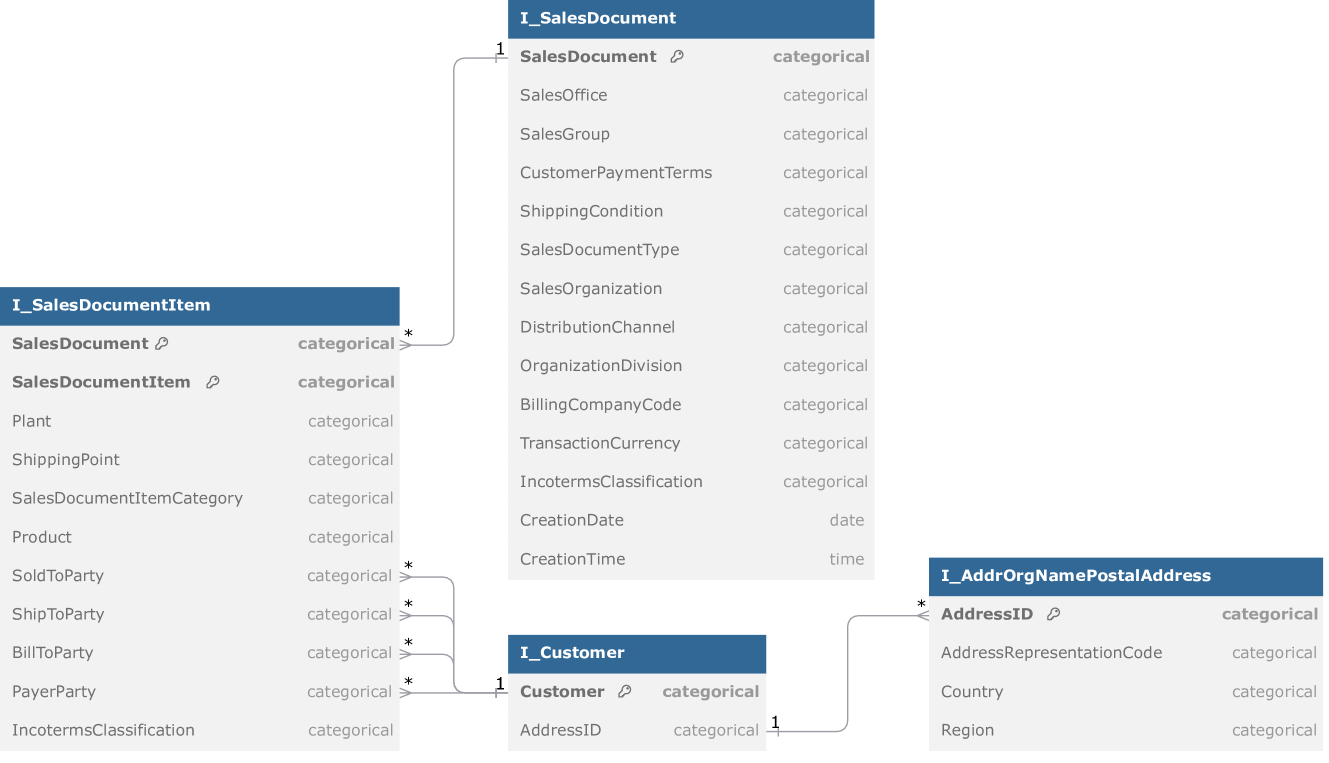
\includegraphics[width=0.75\linewidth]{figures/salt_schema.png}
    \caption{\relbench schema of the newly added Sales Autocompletion Linked Business Tables (SALT) dataset~\citep{sap-salt}.}
    \label{fig:salt-schema}
\end{figure}


\begin{figure}[!ht]
    \centering
    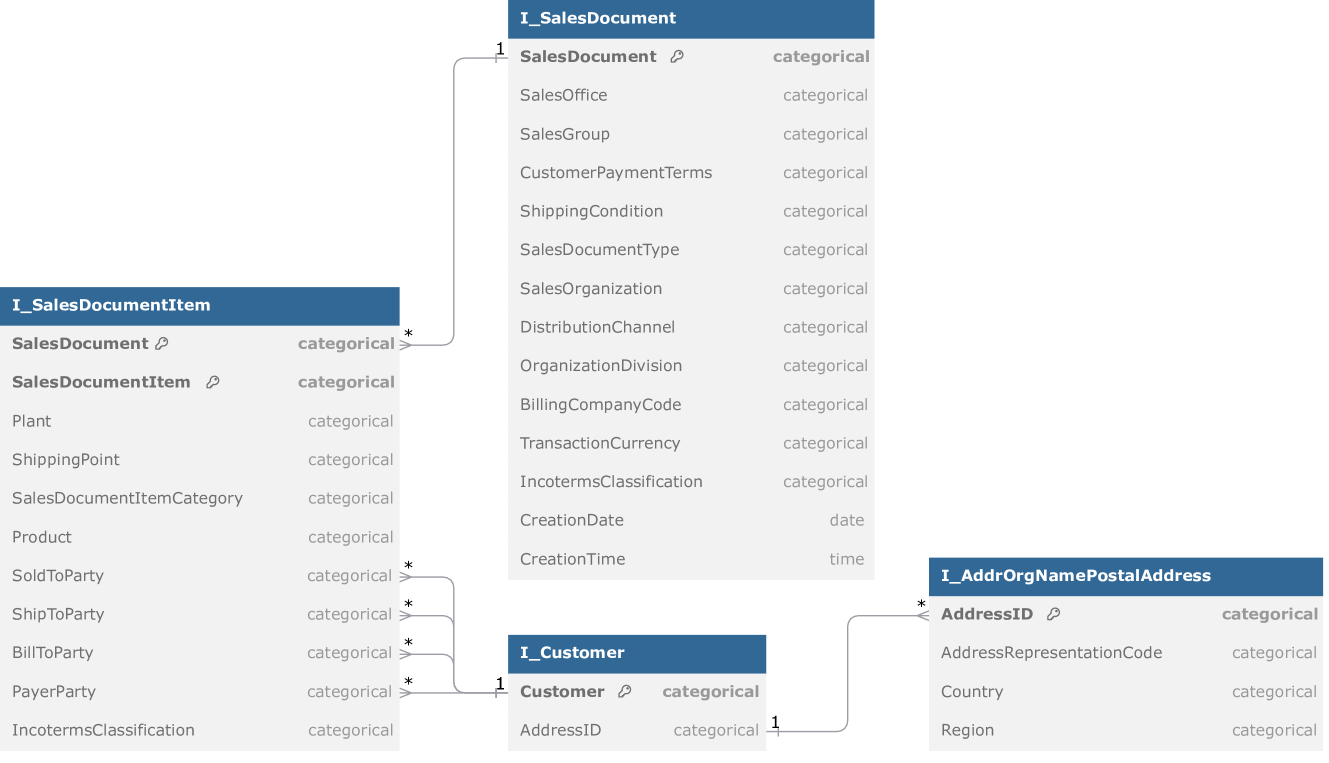
\includegraphics[width=0.75\linewidth]{figures/salt_schema.png}
    \caption{\relbench schema of the newly added arXiv-physics dataset~\citep{arxiv_physics_dataset}.}
    \label{fig:arxiv-schema}
\end{figure}

\begin{figure}[!ht]
    \centering
    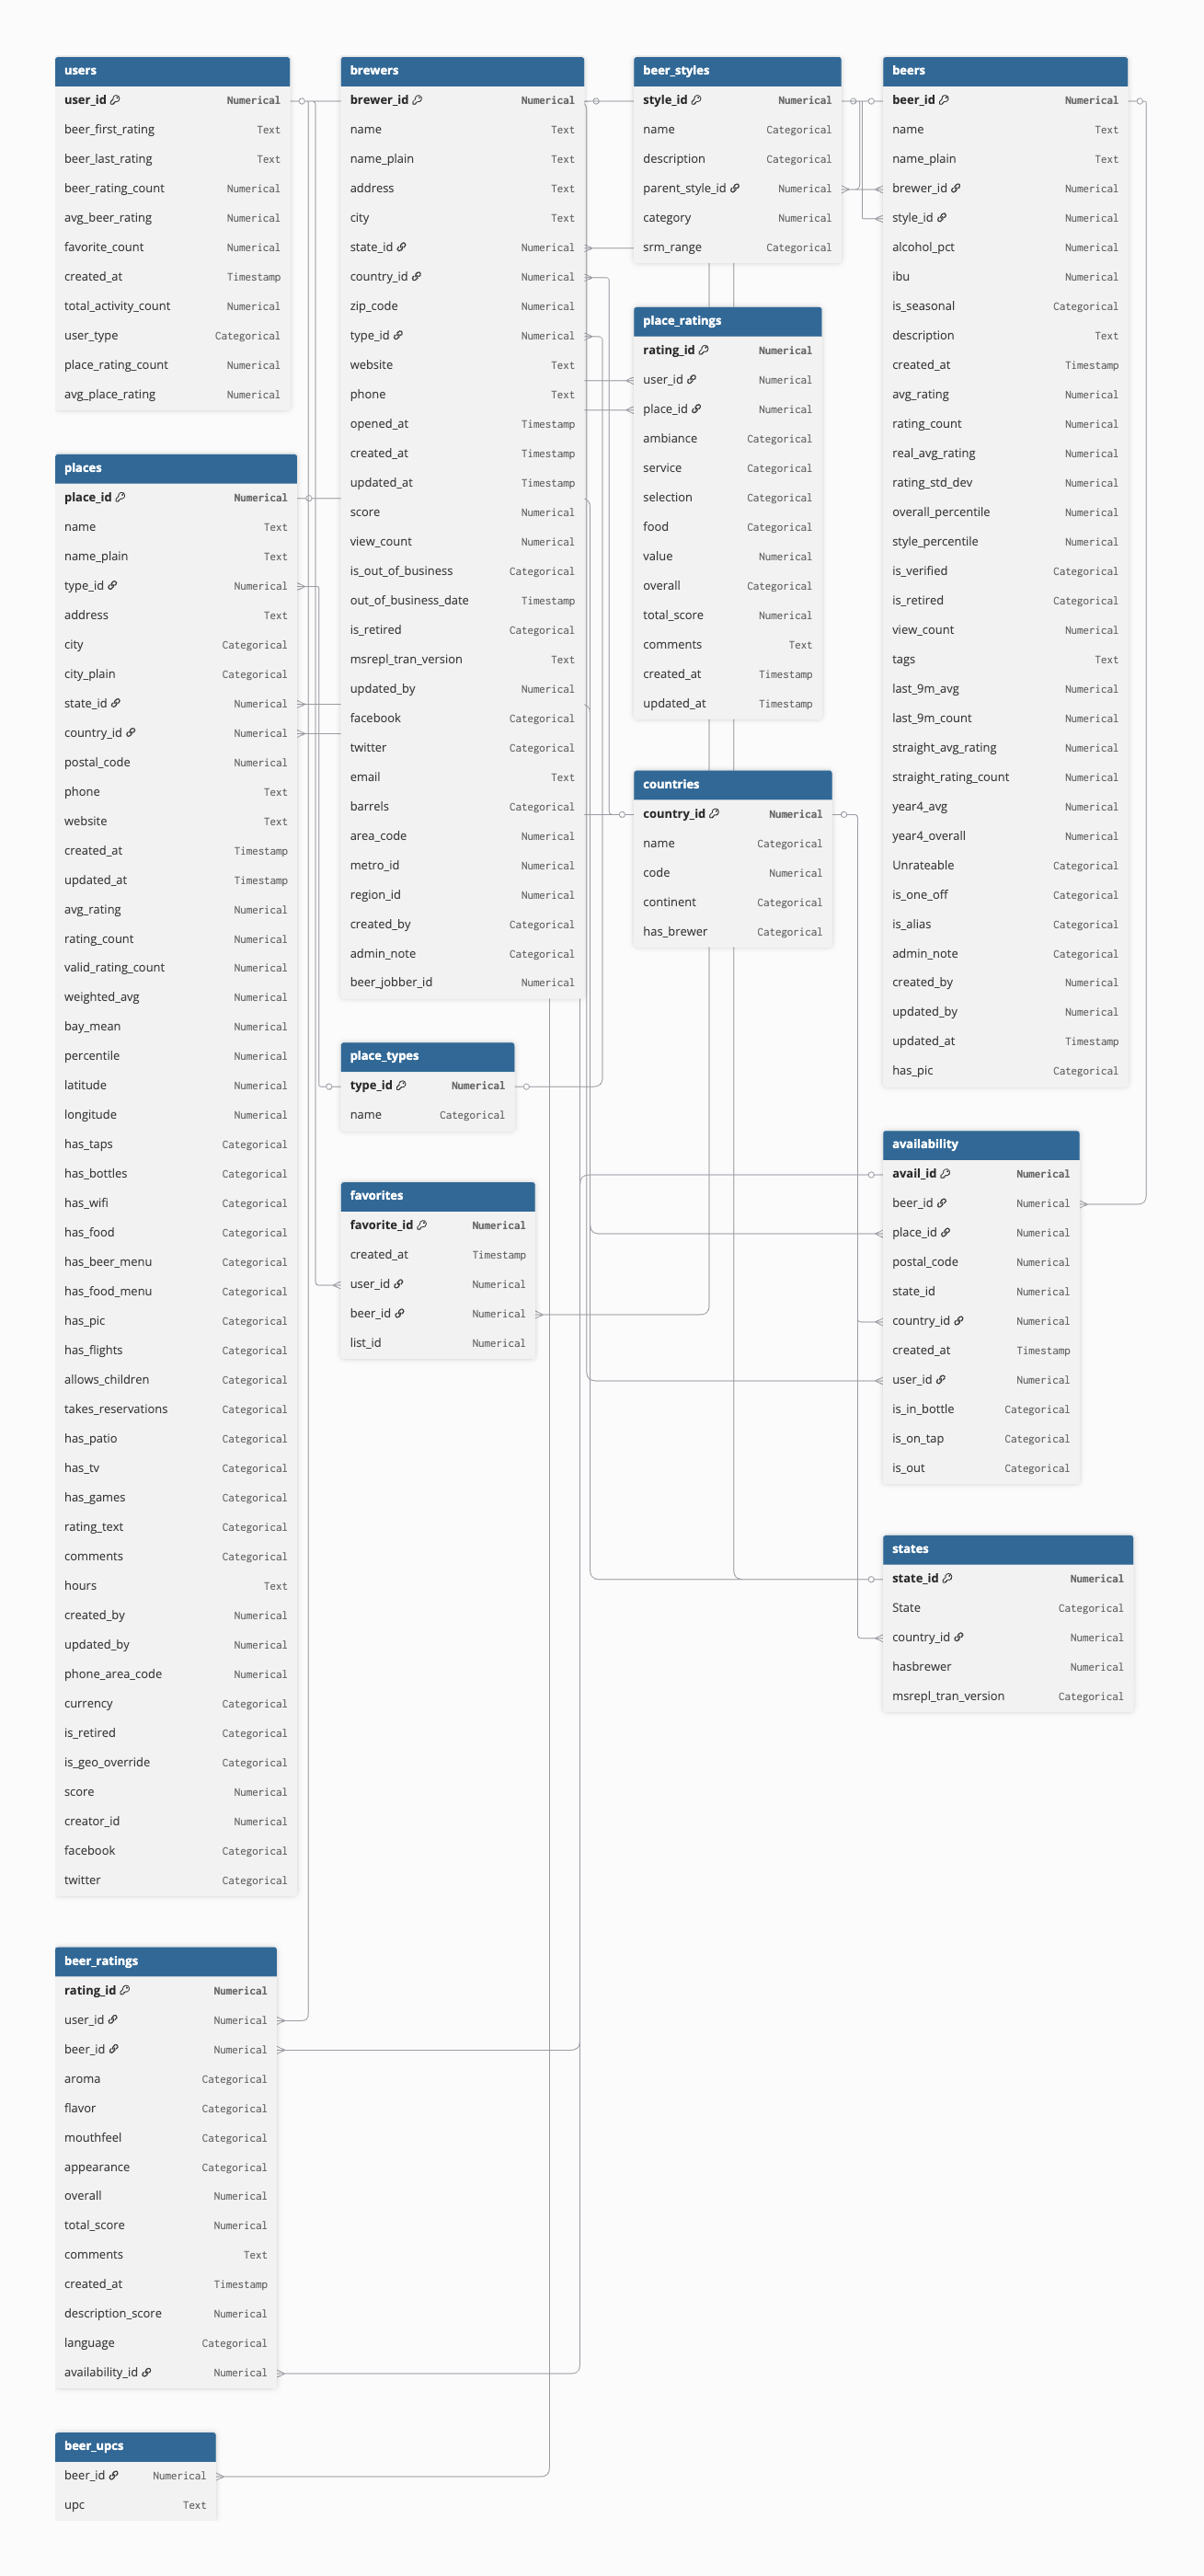
\includegraphics[width=0.7\linewidth]{figures/ratebeer_schema.png}
    \caption{\relbench schema of the newly added RateBeer dataset.}
    \label{fig:ratebeer-schema}
\end{figure}

\begin{figure}[!ht]
    \centering
    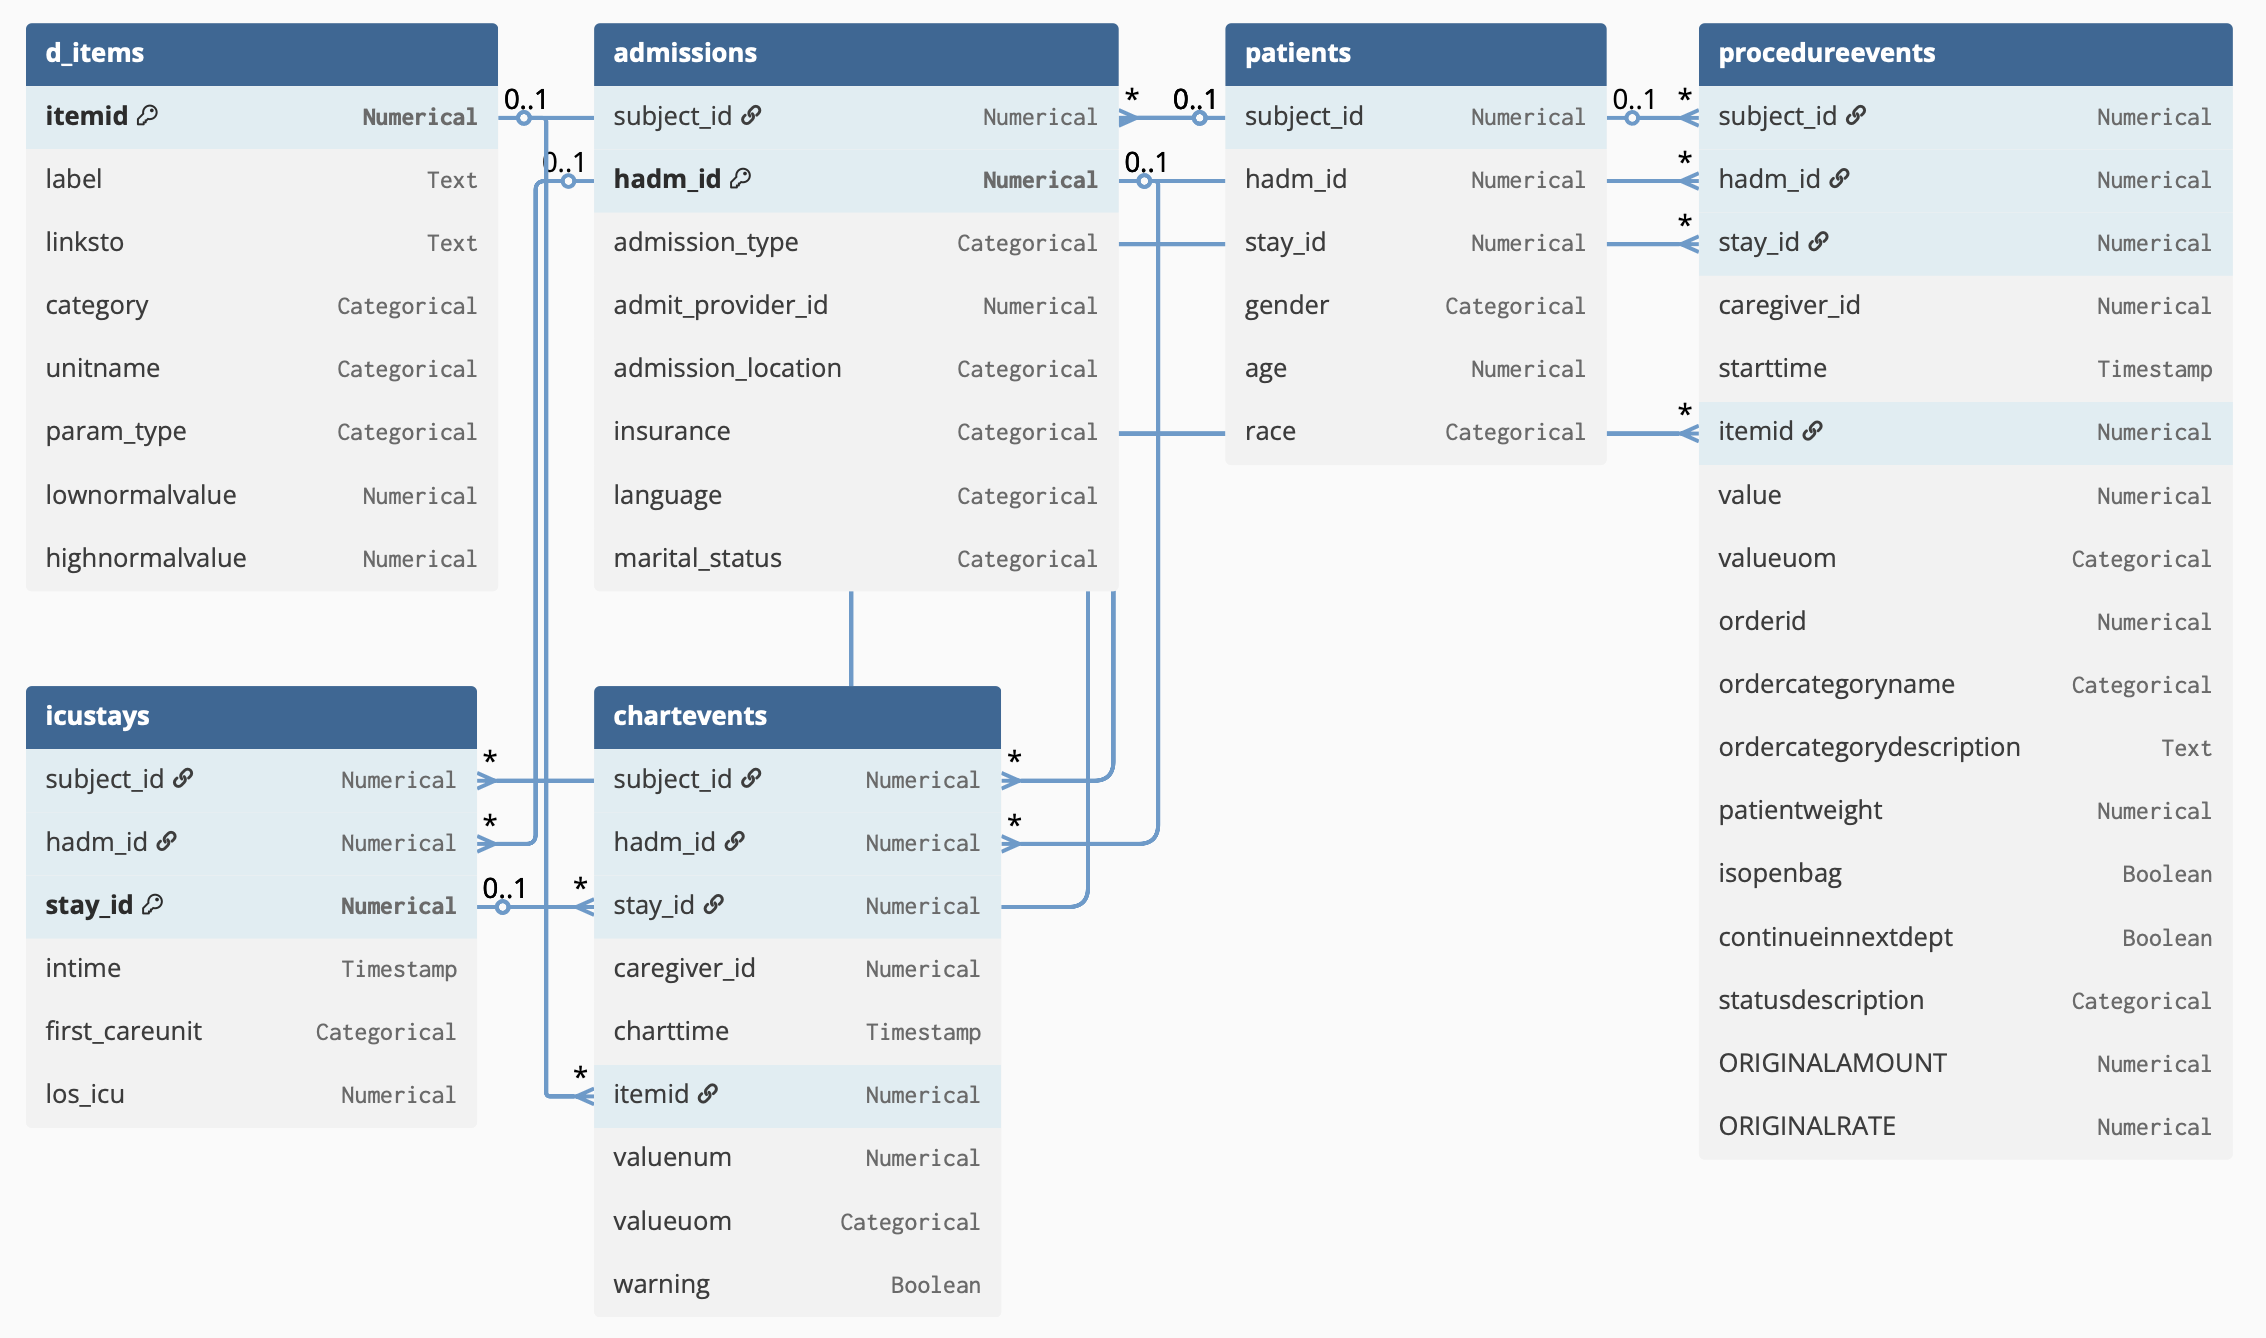
\includegraphics[width=0.7\linewidth]{figures/mimic_schema.png}
    \caption{\relbench schema of the newly added MIMIC-IV v3.1 dataset~\citep{johnson2024mimic}.}
    \label{fig:ratebeer-schema}
\end{figure}


\newpage

\section{Additional Task Information} \label{sec:task_info}


\subsection{Autocomplete task: motivation}

Autocomplete tasks were inspired by the sales order autocomplete task from the SAP S/4HANA Sales
Order User interface. In Figure \ref{fig:autocomplete-example}, the response fields as a whole correspond to one row in a dataset. The user has filled in most of the response fields, allowing the interface to predict the terms of payment for this record.

\begin{figure}[!ht]
    \centering
    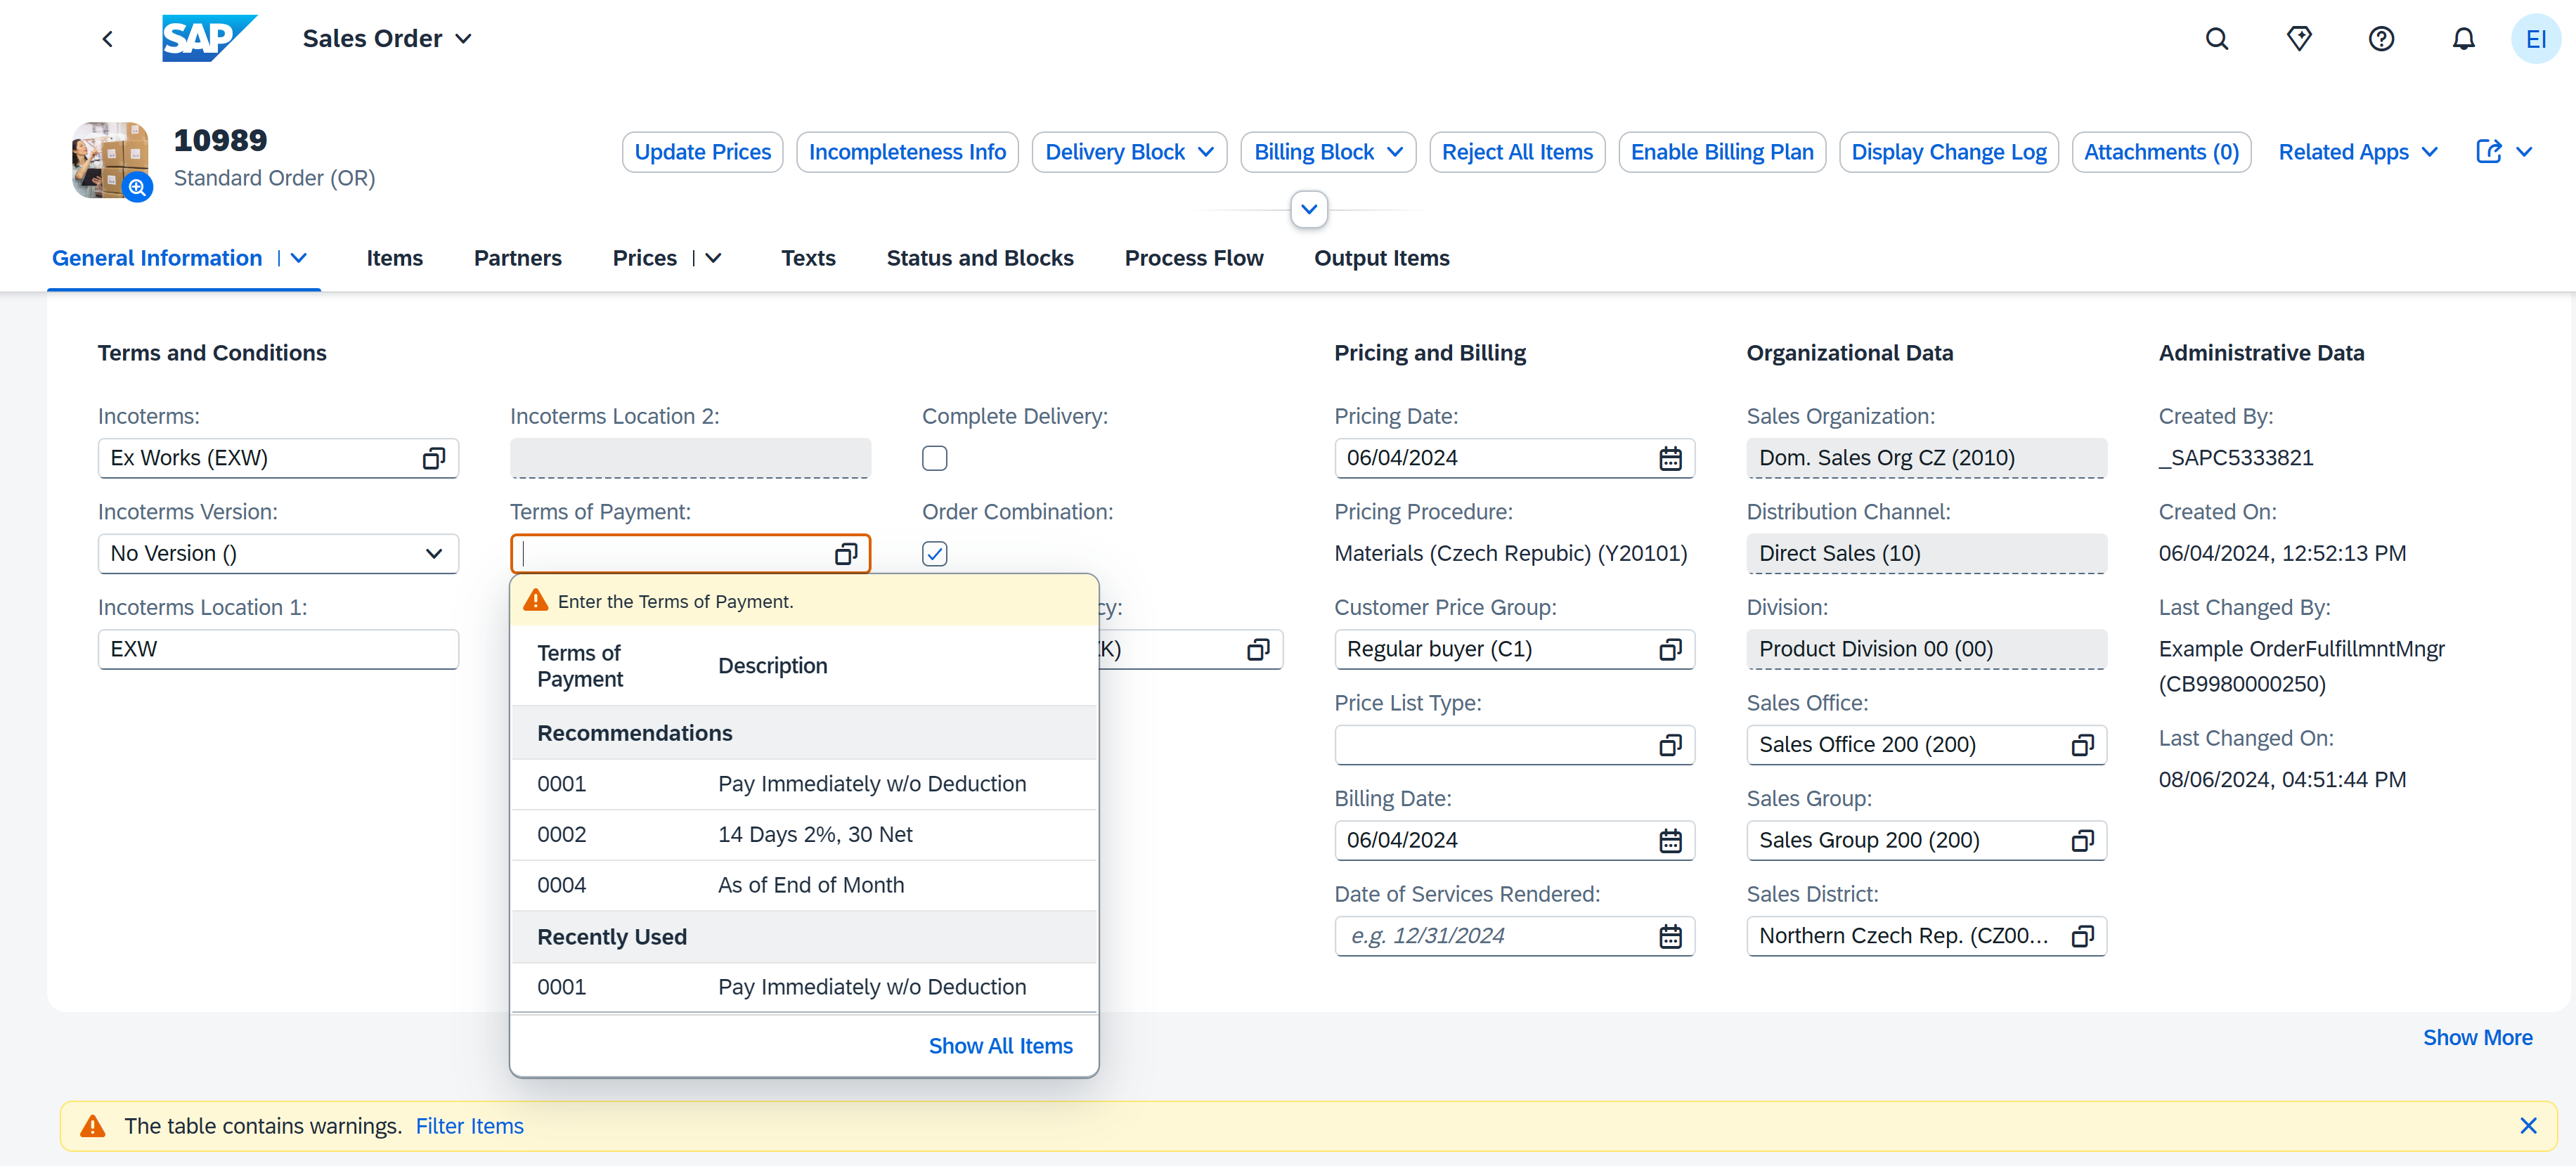
\includegraphics[width=0.8\linewidth]{figures/autocomplete_task.png}
    \caption{Illustrative example of a real-world autocomplete task, where the SAP S/4HANA Sales Order User interface \citep{sap-salt} predicts payment terms based on other filled-in response fields.}
    \label{fig:autocomplete-example}
\end{figure}


\subsection{List of predictive task descriptions}

\begin{enumerate}
  \item \texttt{rel-amazon}
    
    Autocomplete Regression:
    \begin{itemize}
      \item \texttt{review-rating}: For each review, predict the star rating.
    \end{itemize}


  \item \texttt{rel-arxiv}

  Forecasting Classification:
  \begin{itemize}
    \item \texttt{paper-citation}: For each paper, predict whether it will receive at least one citation in the next 6 months.
    \item \texttt{author-category}: For each author, predict the primary research category in which they will publish most in the next 6 months.
  \end{itemize}

  Forecasting Regression:
  \begin{itemize}
    \item \texttt{author-publication}: For each author, predict how many papers they will publish in the next 6 months.
  \end{itemize}

  Recommendation:
  \begin{itemize}
    \item \texttt{paper-paper-cocitation}: For each paper, predict which other papers will be co-cited with it in the next 6 months.
  \end{itemize}

  \item \texttt{rel-avito}

  Autocomplete Classification:
  \begin{itemize}
    \item \texttt{searchstream-click}: For each search session, predict whether the user clicked on a result.
    \item \texttt{searchinfo-isuserloggedon}: For each search, predict whether the user was logged in.
  \end{itemize}


  \item \texttt{rel-trial}

  Autocomplete Classification:
  \begin{itemize}
    \item \texttt{studies-has\_dmc}: For each study, predict whether it has a data monitoring committee.
    \item \texttt{eligibilities-adult}: For each study, predict whether it includes adult participants.
    \item \texttt{eligibilities-child}: For each study, predict whether it includes child participants.
  \end{itemize}

  Autocomplete Regression:
  \begin{itemize}
    \item \texttt{studies-enrollment}: For each study, predict the enrollment count.
  \end{itemize}


  \item \texttt{rel-event}

  Autocomplete Classification:
  \begin{itemize}
    \item \texttt{event\_interest-interested}: For each user--event interaction, predict whether the user marked the event as ``interested.''
    \item \texttt{event\_interest-not\_interested}: For each user--event interaction, predict whether the user marked the event as ``not interested.''
  \end{itemize}

  Autocomplete Regression:
  \begin{itemize}
    \item \texttt{users-birthyear}: For each user, predict the user's birth year.
  \end{itemize}


  \item \texttt{rel-f1}

  Autocomplete Regression:
  \begin{itemize}
    \item \texttt{results-position}: For each race result, predict the finishing position.
    \item \texttt{qualifying-position}: For each qualifying entry, predict the qualifying position.
  \end{itemize}

  Recommendation:
  \begin{itemize}
    \item \texttt{driver-circuit-compete}: Predict in which circuits a driver will compete in the next year.
  \end{itemize}

  \item \texttt{rel-hm} 

  Autocomplete Regression:
  \begin{itemize}
    \item \texttt{transactions-price}: For each transaction, predict the item price.
  \end{itemize}

  \item \texttt{rel-ratebeer} 

  Autocomplete Regression:
  \begin{itemize}
    \item \texttt{beer\_ratings-total\_score}: For each user, given a beer, predict the total score rating the user will give to the beer.
  \end{itemize}

  Forecasting Classification:
  \begin{itemize}
    \item \texttt{beer-churn}: For each beer, predict if it will receive zero ratings in the next 90 days.
    \item \texttt{user-churn}: For each active user, predict if they will rate zero beers in the next 90 days.
    \item \texttt{brewer-dormant}: For each brewer, predict if it will release zero beers in the next year (risk of going dormant).
  \end{itemize}

  Forecasting Regression:
  \begin{itemize}
    \item \texttt{user-count}: Predict the number of ratings a user will give in the next 90 days.
  \end{itemize}

  Recommendation:
  \begin{itemize}
    \item \texttt{user-beer-favorite}: For each user, predict the top 10 beers they will next add to their Favorites list.
    \item \texttt{user-beer-liked}: For each user, predict the top 10 beers they will rate at least 4.0 / 5.0.
    \item \texttt{user-place-liked}: For each user, predict the top 10 places they will rate at least 80 / 100.
  \end{itemize}

  \item \texttt{rel-salt}

  Autocomplete Classification:
  \begin{itemize}
    \item \texttt{item-plant}: For each sales order item, predict its plant (production/storage facility).
    \item \texttt{item-shippoint}: For each sales order item, predict its shipping point (dispatch location).
    \item \texttt{item-incoterms}: For each sales order item, predict its item-level international commercial terms.
    \item \texttt{sales-office}: For each sales order, predict the sales office responsible for managing sales activities for the relevant products and geographic region.
    \item \texttt{sales-group}: For each sales order, predict the sales group, i.e. the subdivision within the distribution chain that handles the customer and transaction.
    \item \texttt{sales-payterms}: For each sales order, predict the customer payment terms (payment deadlines/discounts).
    \item \texttt{sales-shipcond}: For each sales order, predict the shipping condition (logistics terms).
    \item \texttt{sales-incoterms}: Predict the header-level Incoterms (international commercial terms) for each sales order.
  \end{itemize}


  \item \texttt{rel-stack} 

  Autocomplete Classification:
  \begin{itemize}
    \item \texttt{badges-class}: For each badge, predict the badge class.
  \end{itemize}


  \item \texttt{rel-mimic} 

  Forecasting Classification:
  \begin{itemize}
    \item \texttt{patient-iculengthofstay}: For each patient admitted into the ICU, predict whether their stay will last at least 3 days.
  \end{itemize}

\end{enumerate}



\newpage

\section{Additional results and experiment details} \label{sec:appendix_task_results}


\subsection{Results with standard deviations}

Tables \ref{tab:autocomplete_classification_appendix} - \ref{tab:recommendation_appendix} show mean and standard deviations over 5 runs for the autocomplete classification, autocomplete regression, entity classification, entity regression and link prediction results for all new tasks introduced in \relbench v2. For regression tasks, MAE metrics are reported below (the main paper reports $R^2$ metrics).

%% AUTOCOMPLETE CLASSIFICATION RESULTS MAIN %%
\begin{table}[!ht]
  \centering
  \caption{{\bf Autocomplete binary classification results on \relbench.} Binary classification uses the AUROC metric (higher is better). Standard baselines of random choice and majority class both correspond to AUROC values of approximately 50.00, so we exclude them below. Best values are in bold.}
  \label{tab:autocomplete_classification_appendix}
  \renewcommand{\arraystretch}{1.1}
  \scriptsize
  \resizebox{\textwidth}{!}{
    \begin{tabular}{lllrr}
\toprule
Dataset & Task & Split & LightGBM & GNN \\
\midrule
\multirow[c]{4}{*}{\texttt{rel-avito}} & \multirow[c]{2}{*}{\texttt{searchinfo-isuserloggedon}} & Val & $59.09_{\pm 0.37}$ & $\bm{82.57}_{\pm 0.64}$ \\
 &  & Test & $50.00_{\pm 0.00}$ & $\bm{73.00}_{\pm 0.79}$ \\
\cmidrule{2-5}
 & \multirow[c]{2}{*}{\texttt{searchstream-click}} & Val & $\bm{68.33}_{\pm 0.19}$ & $50.39_{\pm 0.22}$ \\
 &  & Test & $49.92_{\pm 0.17}$ & $\bm{55.92}_{\pm 14.04}$ \\
\cmidrule{1-5} \cmidrule{2-5}
\multirow[c]{4}{*}{\texttt{rel-event}} & \multirow[c]{2}{*}{\texttt{event\_interest-interested}} & Val & $51.25_{\pm 0.00}$ & $\bm{54.16}_{\pm 1.75}$ \\
 &  & Test & $49.57_{\pm 0.00}$ & $47.64_{\pm 3.44}$ \\
\cmidrule{2-5}
 & \multirow[c]{2}{*}{\texttt{event\_interest-not\_interested}} & Val & $51.98_{\pm 0.00}$ & $49.74_{\pm 13.71}$ \\
 &  & Test & $52.88_{\pm 0.00}$ & $\bm{60.40}_{\pm 19.57}$ \\
\cmidrule{1-5} \cmidrule{2-5}
\multirow[c]{6}{*}{\texttt{rel-trial}} & \multirow[c]{2}{*}{\texttt{eligibilities-adult}} & Val & $58.10_{\pm 0.23}$ & $\bm{94.91}_{\pm 0.10}$ \\
 &  & Test & $50.00_{\pm 0.00}$ & $\bm{93.73}_{\pm 0.15}$ \\
\cmidrule{2-5}
 & \multirow[c]{2}{*}{\texttt{eligibilities-child}} & Val & $59.78_{\pm 0.15}$ & $\bm{85.91}_{\pm 0.20}$ \\
 &  & Test & $50.00_{\pm 0.00}$ & $\bm{87.25}_{\pm 0.10}$ \\
\cmidrule{2-5}
 & \multirow[c]{2}{*}{\texttt{studies-has\_dmc}} & Val & $76.47_{\pm 0.26}$ & $\bm{78.21}_{\pm 0.12}$ \\
 &  & Test & $50.00_{\pm 0.00}$ & $\bm{75.72}_{\pm 0.11}$ \\
% \cmidrule{1-5} \cmidrule{2-5}
\bottomrule
\end{tabular}

  }
  \vspace{-10pt}
\end{table}


\begin{table}[!ht]
  \centering
  \caption{{\bf Autocomplete multiclass classification results on \relbench.} Multiclass classification uses the accuracy metric (higher is better). Best values are in bold.}
  \label{tab:autocomplete_multiclass_appendix}
  \renewcommand{\arraystretch}{1.1}
  \scriptsize
  % \resizebox{\textwidth}{!}{
    \begin{tabular}{lllrrrr}
\toprule
Dataset & Task & Split & Random & Majority & LightGBM & GNN \\
\midrule
\multirow[c]{17}{*}{\texttt{rel-salt}} & \multirow[c]{2}{*}{\texttt{item-incoterms}} & Val & $34.49$ & $66.46$ & $66.43_{\pm 0.01}$ & $\bm{80.23}_{\pm 0.48}$ \\
 &  & Test & $30.33$ & $58.05$ & $58.05_{\pm 0.00}$ & $\bm{69.36}_{\pm 0.77}$ \\
\cmidrule{2-7}
 & \multirow[c]{2}{*}{\texttt{item-plant}} & Val & $33.19$ & $60.95$ & $60.97_{\pm 0.04}$ & $\bm{99.70}_{\pm 0.16}$ \\
 &  & Test & $32.38$ & $59.69$ & $59.69_{\pm 0.00}$ & $\bm{99.46}_{\pm 0.12}$ \\
\cmidrule{2-7}
 & \multirow[c]{2}{*}{\texttt{item-shippoint}} & Val & $8.20$ & $2.34$ & $4.72_{\pm 0.02}$ & $\bm{98.54}_{\pm 0.13}$ \\
 &  & Test & $6.53$ & $1.99$ & $5.67_{\pm 5.18}$ & $\bm{98.39}_{\pm 0.08}$ \\
\cmidrule{2-7}
 & \multirow[c]{2}{*}{\texttt{sales-group}} & Val & $0.90$ & $0.86$ & $0.70_{\pm 0.12}$ & $\bm{18.43}_{\pm 0.22}$ \\
 &  & Test & $0.85$ & $0.75$ & $0.94_{\pm 1.32}$ & $\bm{15.76}_{\pm 0.30}$ \\
\cmidrule{2-7}
 & \multirow[c]{2}{*}{\texttt{sales-incoterms}} & Val & $31.83$ & $61.00$ & $60.53_{\pm 0.09}$ & $\bm{69.07}_{\pm 1.46}$ \\
 &  & Test & $29.39$ & $56.63$ & $56.63_{\pm 0.00}$ & $\bm{62.23}_{\pm 0.53}$ \\
\cmidrule{2-7}
 & \multirow[c]{2}{*}{\texttt{sales-office}} & Val & $50.01$ & $\bm{99.91}$ & $99.90_{\pm 0.00}$ & $99.91_{\pm 0.00}$ \\
 &  & Test & $49.71$ & $\bm{99.88}$ & $59.93_{\pm 54.71}$ & $99.88_{\pm 0.00}$ \\
\cmidrule{2-7}
 & \multirow[c]{2}{*}{\texttt{sales-payterms}} & Val & $0.32$ & $0.65$ & $1.85_{\pm 0.33}$ & $\bm{39.88}_{\pm 0.19}$ \\
 &  & Test & $0.24$ & $0.47$ & $5.64_{\pm 5.14}$ & $\bm{37.47}_{\pm 0.43}$ \\
\cmidrule{2-7}
 & \multirow[c]{2}{*}{\texttt{sales-shipcond}} & Val & $16.49$ & $27.61$ & $31.92_{\pm 0.04}$ & $\bm{59.21}_{\pm 1.87}$ \\
 &  & Test & $15.64$ & $26.30$ & $4.91_{\pm 0.00}$ & $\bm{56.85}_{\pm 1.32}$ \\
\cmidrule{1-7} \cmidrule{2-7}
\multirow[c]{2}{*}{\texttt{rel-stack}} & \multirow[c]{2}{*}{\texttt{badges-class}} & Val & $11.59$ & $20.68$ & $1.93_{\pm 0.13}$ & $\bm{79.97}_{\pm 0.05}$ \\
 &  & Test & $10.49$ & $18.34$ & $2.51_{\pm 0.00}$ & $\bm{82.83}_{\pm 0.18}$ \\
% \cmidrule{1-7} \cmidrule{2-7}
\bottomrule
\end{tabular}

  % }
  \vspace{-10pt}
\end{table}

\begin{table}[!ht]
  \centering
  \caption{{\bf Autocomplete regression $R^2$ results on \relbench.} Regression uses the $R^2$ metric (higher is better). Best values are in bold.}
  \label{tab:autocomplete_regression_r2_appendix}
  \renewcommand{\arraystretch}{1.1}
  \scriptsize
    \resizebox{\textwidth}{!}{
    \begin{tabular}{llllllllll}
\toprule
 &  &  & Zero & Mean & Median & Ent. Mean & Ent. Med. & LightGBM & GNN \\
\midrule
\multirow[c]{2}{*}{\texttt{rel-amazon}} & \multirow[c]{2}{*}{\texttt{review-rating}} & Val & $-20.848$ & $\bm{-0.006}$ & $-0.364$ & $-20.848$ & $-20.848$ & $-0.364_{\pm 0.000}$ & $-0.356_{\pm 0.012}$ \\
 &  & Test & $-22.579$ & $\bm{-0.014}$ & $-0.341$ & $-13.313$ & $-13.313$ & $-0.341_{\pm 0.000}$ & $-0.331_{\pm 0.013}$ \\
\cmidrule{1-10} \cmidrule{2-10}
\multirow[c]{2}{*}{\texttt{rel-event}} & \multirow[c]{2}{*}{\texttt{users-birthyear}} & Val & $-55012.323$ & $-0.047$ & $-0.216$ & $-55012.323$ & $-55012.323$ & $0.004_{\pm 0.004}$ & $\bm{0.008}_{\pm 0.036}$ \\
 &  & Test & $-64803.758$ & $-0.121$ & $-0.395$ & $-64803.758$ & $-64803.758$ & $-0.192_{\pm 0.108}$ & $\bm{-0.030}_{\pm 0.040}$ \\
\cmidrule{1-10} \cmidrule{2-10}
 \multirow[c]{4}{*}{\texttt{rel-f1}} & \multirow[c]{2}{*}{\texttt{qualifying-position}} & Val & $-3.267$ & $-0.018$ & $-0.030$ & $-3.267$ & $-3.267$ & $\bm{0.153}_{\pm 0.003}$ & $0.015_{\pm 0.009}$ \\
 &  & Test & $-3.214$ & $-0.002$ & $-0.001$ & $-3.214$ & $-3.214$ & $-0.953_{\pm 0.039}$ & $\bm{0.015}_{\pm 0.010}$ \\
\cmidrule{2-10}
 & \multirow[c]{2}{*}{\texttt{results-position}} & Val & $-3.123$ & $-0.100$ & $-0.107$ & $-3.123$ & $-3.123$ & $0.283_{\pm 0.006}$ & $\bm{0.440}_{\pm 0.026}$ \\
 &  & Test & $-3.148$ & $-0.176$ & $-0.219$ & $-3.148$ & $-3.148$ & $-2.437_{\pm 0.053}$ & $\bm{0.394}_{\pm 0.039}$ \\
\cmidrule{1-10} \cmidrule{2-10}
\multirow[c]{2}{*}{\texttt{rel-hm}} & \multirow[c]{2}{*}{\texttt{transactions-price}} & Val & $-2.215$ & $-0.065$ & $-0.140$ & $-2.215$ & $-2.215$ & $-0.140_{\pm 0.000}$ & $\bm{0.725}_{\pm 0.003}$ \\
 &  & Test & $-2.329$ & $-0.075$ & $-0.159$ & $-2.329$ & $-2.329$ & $-0.160_{\pm 0.000}$ & $\bm{0.736}_{\pm 0.002}$ \\
\cmidrule{1-10} \cmidrule{2-10}
\multirow[c]{2}{*}{\texttt{rel-ratebeer}} & \multirow[c]{2}{*}{\texttt{user-beer-rating}} & Val & $-23.411$ & $-0.015$ & $-0.004$ & $-23.411$ & $-23.411$ & $-0.004_{\pm 0.000}$ & $\bm{0.448}_{\pm 0.006}$ \\
 &  & Test & $-34.352$ & $-0.031$ & $-0.003$ & $-34.352$ & $-34.352$ & $-0.014_{\pm 0.000}$ & $\bm{0.394}_{\pm 0.010}$ \\
\cmidrule{1-10} \cmidrule{2-10}
\multirow[c]{2}{*}{\texttt{rel-trial}} & \multirow[c]{2}{*}{\texttt{studies-enrollment}} & Val & $-0.001$ & $\bm{-0.000}$ & $-0.001$ & $-0.001$ & $-0.001$ & $-0.001_{\pm 0.000}$ & $-0.000_{\pm 0.000}$ \\
 &  & Test & $-0.000$ & $\bm{-0.000}$ & $-0.000$ & $-0.000$ & $-0.000$ & $-0.000_{\pm 0.000}$ & $-0.000_{\pm 0.000}$ \\
\cmidrule{1-10} \cmidrule{2-10}
\bottomrule
\end{tabular}

    }
  \vspace{10pt}
\end{table}

\begin{table}[!ht]
  \centering
  \caption{{\bf Autocomplete regression results on \relbench.} Regression uses the MAE metric (lower is better). Best values are in bold.}
  \label{tab:autocomplete_regression_appendix}
  \renewcommand{\arraystretch}{1.1}
  \scriptsize
    \resizebox{\textwidth}{!}{
    \begin{tabular}{lllrrrrrrr}
\toprule
Dataset & Task & Split & Zero & Mean & Median & Ent. Mean & Ent. Med. & LightGBM & GNN \\
\midrule
\multirow[c]{2}{*}{\texttt{rel-amazon}} & \multirow[c]{2}{*}{\texttt{review-rating}} & Val & $4.416$ & $0.779$ & $\bm{0.584}$ & $4.416$ & $4.416$ & $0.584_{\pm 0.000}$ & $0.586_{\pm 0.003}$ \\
 &  & Test & $4.453$ & $0.762$ & $\bm{0.547}$ & $2.907$ & $2.907$ & $0.547_{\pm 0.000}$ & $0.549_{\pm 0.004}$ \\
\cmidrule{1-10} \cmidrule{2-10}
\multirow[c]{2}{*}{\texttt{rel-event}} & \multirow[c]{2}{*}{\texttt{users-birthyear}} & Val & $1987.058$ & $5.668$ & $5.885$ & $1987.058$ & $1987.058$ & $\bm{5.144}_{\pm 0.006}$ & $5.193_{\pm 0.044}$ \\
 &  & Test & $1986.094$ & $5.588$ & $6.198$ & $1986.094$ & $1986.094$ & $5.752_{\pm 0.164}$ & $\bm{5.224}_{\pm 0.046}$ \\
\cmidrule{1-10} \cmidrule{2-10}
 \multirow[c]{8}{*}{\texttt{rel-f1}} & \multirow[c]{2}{*}{\texttt{qualifying-position}} & Val & $10.943$ & $5.266$ & $5.280$ & $10.943$ & $10.943$ & $\bm{4.411}_{\pm 0.014}$ & $5.190_{\pm 0.023}$ \\
 &  & Test & $11.142$ & $5.358$ & $5.342$ & $11.142$ & $11.142$ & $7.048_{\pm 0.067}$ & $\bm{5.312}_{\pm 0.023}$ \\
\cmidrule{2-10}
 & \multirow[c]{2}{*}{\texttt{results-position}} & Val & $8.587$ & $4.251$ & $4.257$ & $8.587$ & $8.587$ & $3.167_{\pm 0.014}$ & $\bm{2.779}_{\pm 0.069}$ \\
 &  & Test & $9.504$ & $4.822$ & $4.877$ & $9.504$ & $9.504$ & $8.377_{\pm 0.080}$ & $\bm{3.139}_{\pm 0.104}$ \\
\cmidrule{1-10} \cmidrule{2-10}
\multirow[c]{2}{*}{\texttt{rel-hm}} & \multirow[c]{2}{*}{\texttt{transactions-price}} & Val & $0.034$ & $0.015$ & $0.015$ & $0.034$ & $0.034$ & $0.015_{\pm 0.000}$ & $\bm{0.004}_{\pm 0.000}$ \\
 &  & Test & $0.034$ & $0.015$ & $0.015$ & $0.034$ & $0.034$ & $0.015_{\pm 0.000}$ & $\bm{0.004}_{\pm 0.000}$ \\
\cmidrule{1-10} \cmidrule{2-10}
\multirow[c]{2}{*}{\texttt{rel-ratebeer}} & \multirow[c]{2}{*}{\texttt{beer\_ratings-total\_score}} & Val & $3.444$ & $0.530$ & $0.520$ & $3.444$ & $3.444$ & $0.520_{\pm 0.000}$ & $\bm{0.355}_{\pm 0.001}$ \\
 &  & Test & $3.470$ & $0.457$ & $0.431$ & $3.470$ & $3.470$ & $0.447_{\pm 0.000}$ & $\bm{0.323}_{\pm 0.003}$ \\
\cmidrule{1-10} \cmidrule{2-10}
\multirow[c]{2}{*}{\texttt{rel-trial}} & \multirow[c]{2}{*}{\texttt{studies-enrollment}} & Val & $3782.463$ & $5893.531$ & $3754.731$ & $3782.463$ & $3782.463$ & $3734.843_{\pm 1.368}$ & $\bm{3709.484}_{\pm 1.698}$ \\
 &  & Test & $17660.073$ & $19949.874$ & $17635.281$ & $17660.073$ & $17660.073$ & $17770.098_{\pm 72.701}$ & $\bm{17604.633}_{\pm 1.562}$ \\
% \cmidrule{1-10} \cmidrule{2-10}
\bottomrule
\end{tabular}

    }
  \vspace{10pt}
\end{table}


\begin{table}[!ht]
  \centering
  \caption{{\bf Entity binary classification results on \relbench.} Binary classification uses the AUROC metric (higher is better). Standard baselines of random choice and majority class both correspond to AUROC values of approximately 50.00, so we exclude them below. Best values are in bold.}
  \label{tab:entity_classification_appendix}
  \renewcommand{\arraystretch}{1.1}
  \scriptsize
    % \resizebox{\textwidth}{!}{
    \begin{tabular}{lllrr}
\toprule
Dataset & Task & Split & LightGBM & GNN \\
\midrule
\multirow[c]{2}{*}{\texttt{rel-arxiv}} & \multirow[c]{2}{*}{\texttt{paper-citation}} & Val & $71.94_{\pm 0.12}$ & $\bm{82.45}_{\pm 0.03}$ \\
 &  & Test & $71.21_{\pm 0.13}$ & $\bm{82.50}_{\pm 0.04}$ \\
\cmidrule{1-5} \cmidrule{2-5}
\multirow[c]{2}{*}{\texttt{rel-mimic}} & \multirow[c]{2}{*}{\texttt{patient-iculengthofstay}} & Val & $53.64_{\pm 0.28}$ & $\bm{56.52}_{\pm 0.05}$ \\
 &  & Test & $51.81_{\pm 0.56}$ & $\bm{55.01}_{\pm 0.11}$ \\
\cmidrule{1-5} \cmidrule{2-5}
\multirow[c]{6}{*}{\texttt{rel-ratebeer}} & \multirow[c]{2}{*}{\texttt{beer-churn}} & Val & $81.90_{\pm 0.06}$ & $\bm{90.47}_{\pm 0.06}$ \\
 &  & Test & $76.21_{\pm 0.12}$ & $\bm{78.67}_{\pm 0.60}$ \\
\cmidrule{2-5}
 & \multirow[c]{2}{*}{\texttt{brewer-dormant}} & Val & $76.39_{\pm 0.10}$ & $\bm{82.10}_{\pm 0.13}$ \\
 &  & Test & $75.79_{\pm 0.11}$ & $\bm{80.51}_{\pm 0.17}$ \\
\cmidrule{2-5}
 & \multirow[c]{2}{*}{\texttt{user-churn}} & Val & $87.02_{\pm 0.02}$ & $\bm{96.85}_{\pm 0.26}$ \\
 &  & Test & $83.92_{\pm 18.42}$ & $\bm{94.27}_{\pm 0.22}$ \\
% \cmidrule{1-5} \cmidrule{2-5}
\bottomrule
\end{tabular}

    % } 
  \vspace{10pt}
\end{table}

\begin{table}[!ht]
  \centering
  \caption{{\bf Entity multiclass classification results on \relbench.} Multiclass classification uses the accuracy metric (higher is better). Best values are in bold.}
  \label{tab:entity_multiclass_appendix}
  \renewcommand{\arraystretch}{1.1}
  \scriptsize
    % \resizebox{\textwidth}{!}{
    \begin{tabular}{lllrrrr}
\toprule
Dataset & Task & Split & Random & Majority & LightGBM & GNN \\
\midrule
\multirow[c]{2}{*}{\texttt{rel-arxiv}} & \multirow[c]{2}{*}{\texttt{author-category}} & Val & $1.75$ & $8.83$ & $1.95_{\pm 0.16}$ & $\bm{52.63}_{\pm 0.08}$ \\
 &  & Test & $1.77$ & $9.09$ & $2.01_{\pm 0.21}$ & $\bm{50.74}_{\pm 1.01}$ \\
% \cmidrule{1-7} \cmidrule{2-7}
\bottomrule
\end{tabular}

    % } 
  \vspace{10pt}
\end{table}

\begin{table}[!ht]
  \centering
  \caption{{\bf Entity regression $R^2$ results on \relbench.} Regression uses the $R^2$ metric (higher is better). Best values are in bold.}
  \label{tab:entity_regression_r2_appendix}
  \renewcommand{\arraystretch}{1.1}
  \scriptsize
    \resizebox{\textwidth}{!}{
    \begin{tabular}{llllllllll}
\toprule
 &  &  & Zero & Mean & Median & Ent. Mean & Ent. Med. & LightGBM & GNN \\
\midrule
\multirow[c]{4}{*}{\texttt{rel-amazon}} & \multirow[c]{2}{*}{\texttt{item-ltv}} & Val & $-0.025$ & $-0.000$ & $-0.013$ & $-0.247$ & $-0.107$ & $0.002_{\pm 0.001}$ & $\bm{0.066}_{\pm 0.003}$ \\
 &  & Test & $-0.013$ & $-0.000$ & $-0.007$ & $0.030$ & $\bm{0.099}$ & $0.001_{\pm 0.000}$ & $0.032_{\pm 0.001}$ \\
\cmidrule{2-10}
 & \multirow[c]{2}{*}{\texttt{user-ltv}} & Val & $-0.084$ & $-0.003$ & $-0.084$ & $0.053$ & $0.095$ & $-0.084_{\pm 0.000}$ & $\bm{0.195}_{\pm 0.006}$ \\
 &  & Test & $-0.092$ & $-0.000$ & $-0.092$ & $0.143$ & $0.168$ & $-0.092_{\pm 0.000}$ & $\bm{0.172}_{\pm 0.006}$ \\
\cmidrule{1-10} \cmidrule{2-10}
\multirow[c]{2}{*}{\texttt{rel-arxiv}} & \multirow[c]{2}{*}{\texttt{author-publication}} & Val & $-1.579$ & $-0.012$ & $-0.259$ & $0.254$ & $0.236$ & $-0.259_{\pm 0.000}$ & $\bm{0.437}_{\pm 0.013}$ \\
 &  & Test & $-1.572$ & $-0.000$ & $-0.210$ & $-0.010$ & $-0.064$ & $-0.210_{\pm 0.000}$ & $\bm{0.249}_{\pm 0.013}$ \\
\cmidrule{1-10} \cmidrule{2-10}
\multirow[c]{2}{*}{\texttt{rel-avito}} & \multirow[c]{2}{*}{\texttt{ad-ctr}} & Val & $-0.238$ & $-0.002$ & $-0.095$ & $-0.224$ & $-0.224$ & $-0.032_{\pm 0.005}$ & $\bm{0.030}_{\pm 0.017}$ \\
 &  & Test & $-0.226$ & $-0.004$ & $-0.098$ & $-0.148$ & $-0.148$ & $-0.039_{\pm 0.004}$ & $\bm{-0.001}_{\pm 0.020}$ \\
\cmidrule{1-10} \cmidrule{2-10}
\multirow[c]{2}{*}{\texttt{rel-event}} & \multirow[c]{2}{*}{\texttt{user-attendance}} & Val & $-0.249$ & $\bm{-0.037}$ & $-0.249$ & $-0.193$ & $-0.147$ & $-0.249_{\pm 0.001}$ & $-0.045_{\pm 0.116}$ \\
 &  & Test & $-0.168$ & $-0.019$ & $-0.168$ & $-0.065$ & $-0.043$ & $-0.168_{\pm 0.000}$ & $\bm{0.003}_{\pm 0.096}$ \\
\cmidrule{1-10} \cmidrule{2-10}
\multirow[c]{2}{*}{\texttt{rel-f1}} & \multirow[c]{2}{*}{\texttt{driver-position}} & Val & $-5.715$ & $-0.370$ & $-0.236$ & $-2.866$ & $-2.840$ & $0.150_{\pm 0.025}$ & $\bm{0.249}_{\pm 0.008}$ \\
 &  & Test & $-5.239$ & $-0.119$ & $-0.042$ & $-2.841$ & $-2.849$ & $\bm{0.068}_{\pm 0.049}$ & $0.039_{\pm 0.063}$ \\
\cmidrule{1-10} \cmidrule{2-10}
\multirow[c]{2}{*}{\texttt{rel-hm}} & \multirow[c]{2}{*}{\texttt{item-sales}} & Val & $-0.017$ & $-0.000$ & $-0.017$ & $0.065$ & $0.053$ & $-0.017_{\pm 0.000}$ & $\bm{0.187}_{\pm 0.002}$ \\
 &  & Test & $-0.017$ & $-0.000$ & $-0.017$ & $0.058$ & $0.042$ & $-0.017_{\pm 0.000}$ & $\bm{0.215}_{\pm 0.002}$ \\
\cmidrule{1-10} \cmidrule{2-10}
\multirow[c]{2}{*}{\texttt{rel-ratebeer}} & \multirow[c]{2}{*}{\texttt{user-count}} & Val & $-0.037$ & $-0.053$ & $-0.037$ & $0.551$ & $0.547$ & $\bm{0.559}_{\pm 0.014}$ & $0.526_{\pm 0.005}$ \\
 &  & Test & $-0.071$ & $-0.025$ & $-0.071$ & $0.264$ & $0.285$ & $-0.170_{\pm 0.684}$ & $\bm{0.625}_{\pm 0.003}$ \\
\cmidrule{1-10} \cmidrule{2-10}
\multirow[c]{2}{*}{\texttt{rel-stack}} & \multirow[c]{2}{*}{\texttt{post-votes}} & Val & $-0.028$ & $-0.007$ & $-0.028$ & $\bm{0.306}$ & $0.285$ & $-0.028_{\pm 0.000}$ & $0.122_{\pm 0.003}$ \\
 &  & Test & $-0.034$ & $-0.004$ & $-0.034$ & $\bm{0.294}$ & $0.272$ & $-0.034_{\pm 0.000}$ & $0.122_{\pm 0.004}$ \\
\cmidrule{1-10} \cmidrule{2-10}
\multirow[c]{4}{*}{\texttt{rel-trial}} & \multirow[c]{2}{*}{\texttt{site-success}} & Val & $-0.988$ & $\bm{-0.005}$ & $-0.988$ & $-0.749$ & $-0.809$ & $-0.319_{\pm 0.077}$ & $-0.425_{\pm 0.059}$ \\
 &  & Test & $-0.923$ & $\bm{-0.001}$ & $-0.923$ & $-0.714$ & $-0.751$ & $-0.336_{\pm 0.087}$ & $-0.483_{\pm 0.110}$ \\
\cmidrule{2-10}
 & \multirow[c]{2}{*}{\texttt{study-adverse}} & Val & $-0.021$ & $-0.002$ & $-0.020$ & $-0.021$ & $-0.021$ & $\bm{0.134}_{\pm 0.017}$ & $0.066_{\pm 0.003}$ \\
 &  & Test & $-0.054$ & $-0.005$ & $-0.050$ & $-0.054$ & $-0.054$ & $\bm{0.307}_{\pm 0.039}$ & $0.177_{\pm 0.009}$ \\
\cmidrule{1-10} \cmidrule{2-10}
\bottomrule
\end{tabular}

    }
  \vspace{10pt}
\end{table}

\begin{table}[!ht]
  \centering
  \caption{{\bf Entity regression results on \relbench.} Regression uses the MAE metric (lower is better). Best values are in bold.}
  \label{tab:entity_regression_appendix}
  \renewcommand{\arraystretch}{1.1}
  \scriptsize
    \resizebox{\textwidth}{!}{
    \begin{tabular}{lllrrrrrrr}
\toprule
Dataset & Task & Split & Zero & Mean & Median & Ent. Mean & Ent. Med. & LightGBM & GNN \\
\midrule
\multirow[c]{2}{*}{\texttt{rel-arxiv}} & \multirow[c]{2}{*}{\texttt{author-publication}} & Val & $1.681$ & $0.864$ & $0.681$ & $0.827$ & $0.804$ & $0.681_{\pm 0.000}$ & $\bm{0.435}_{\pm 0.008}$ \\
 &  & Test & $1.577$ & $0.769$ & $0.577$ & $0.879$ & $0.874$ & $0.577_{\pm 0.000}$ & $\bm{0.513}_{\pm 0.008}$ \\
\cmidrule{1-10} \cmidrule{2-10}
\multirow[c]{2}{*}{\texttt{rel-ratebeer}} & \multirow[c]{2}{*}{\texttt{user-count}} & Val & $11.255$ & $28.892$ & $11.255$ & $8.363$ & $7.866$ & $7.065_{\pm 0.058}$ & $\bm{5.813}_{\pm 0.031}$ \\
 &  & Test & $15.124$ & $29.050$ & $15.124$ & $13.883$ & $13.079$ & $20.350_{\pm 9.536}$ & $\bm{7.374}_{\pm 0.102}$ \\
% \cmidrule{1-10} \cmidrule{2-10}
\bottomrule
\end{tabular}

    }
  \vspace{10pt}
\end{table}



\begin{table}[!ht]
  \centering
  \caption{{\bf Recommendation results on \relbench.} Recommendation uses the MAP metric (higher is better). Best values are in bold.}
  \label{tab:recommendation_appendix}
  \renewcommand{\arraystretch}{1.1}
  \scriptsize
    \resizebox{\textwidth}{!}{
    \begin{tabular}{lllrrrrrrr}
\toprule
Dataset & Task & Split & Past Visit & Global Pop. & LightGBM & GNN (2) & GNN (4) & IDGNN (2) & IDGNN (4) \\
\midrule
\multirow[c]{2}{*}{\texttt{rel-arxiv}} & \multirow[c]{2}{*}{\texttt{paper-paper-cocitation}} & Val & $19.01$ & $1.25$ & $12.49_{\pm 0.60}$ & $12.19_{\pm 0.23}$ & $12.96_{\pm 00.33}$ & $25.22_{\pm 0.09}$ & $\bm{35.76}_{\pm 0.09}$ \\
 &  & Test & $16.51$ & $1.13$ & $11.01_{\pm 0.43}$ & $8.83_{\pm 0.38}$ & $10.46_{\pm 0.56}$ & $22.95_{\pm 0.07}$ & $\bm{35.39}_{\pm 0.17}$ \\
\cmidrule{1-10} \cmidrule{2-10}
\multirow[c]{2}{*}{\texttt{rel-f1}} & \multirow[c]{2}{*}{\texttt{driver-circuit-compete}} & Val & $53.41$ & $55.19$ & $66.06_{\pm 2.68}$ & $3.60_{\pm 2.11}$ & $10.57_{\pm 8.35}$ & $70.70_{\pm 0.00}$ & $\bm{74.40}_{\pm 1.03}$ \\
 &  & Test & $20.76$ & $50.12$ & $57.77_{\pm 2.95}$ & $9.67_{\pm 10.56}$ & $16.57_{\pm 11.17}$ & $62.32_{\pm 0.00}$ & $\bm{76.18}_{\pm 6.59}$ \\
\cmidrule{1-10} \cmidrule{2-10}
\multirow[c]{6}{*}{\texttt{rel-ratebeer}} & \multirow[c]{2}{*}{\texttt{user-beer-favorite}} & Val & $0.00$ & $2.33$ & $1.24_{\pm 0.15}$ & $2.09_{\pm 0.15}$ & $-$ & $3.09_{\pm 0.14}$ & $\bm{3.33}_{\pm 0.09}$ \\
 &  & Test & $0.00$ & $1.10$ & $0.67_{\pm 0.13}$ & $0.56_{\pm 0.22}$ & $-$ & $1.21_{\pm 0.93}$ & $\bm{1.89}_{\pm 0.09}$ \\
\cmidrule{2-10}
 & \multirow[c]{2}{*}{\texttt{user-beer-liked}} & Val & $0.00$ & $0.77$ & $0.43_{\pm 0.02}$ & $0.77_{\pm 0.06}$ & $-$ & $0.21_{\pm 0.01}$ & $1.48_{\pm 0.06}$ \\
 &  & Test & $0.00$ & $0.61$ & $0.29_{\pm 0.04}$ & $0.54_{\pm 0.22}$ & $-$ & $0.32_{\pm 0.03}$ & $1.46_{\pm 0.19}$ \\
\cmidrule{2-10}
 & \multirow[c]{2}{*}{\texttt{user-place-liked}} & Val & $0.00$ & $0.24$ & $0.24_{\pm 0.07}$ & $1.06_{\pm 0.17}$ & $-$ & $0.88_{\pm 0.09}$ & $2.20_{\pm 0.24}$ \\
 &  & Test & $0.00$ & $0.11$ & $0.08_{\pm 0.03}$ & $1.15_{\pm 0.34}$ & $-$ & $0.60_{\pm 0.50}$ & $1.85_{\pm 0.30}$ \\
% \cmidrule{1-10} \cmidrule{2-10}
\bottomrule
\end{tabular}

    }
  \vspace{10pt}
\end{table}


\subsection{Additional regression metrics}

For regression tasks, the main paper reports $R^2$ to measure each method's predictive power, while MAE is reported in Tables \ref{tab:autocomplete_regression_appendix} and \ref{tab:entity_regression_appendix} above.

\newpage

\subsection{Recommendation task ablations}

\textbf{The benefit of node position}. ID-GNN, which strongly utilizes node position, excels in entity-specific tasks. For example, we focus on the \ratebeer dataset whose recommendation tasks strongly highlight user-specific preferences. We observed that ID-GNN significantly outperforms plain GraphSAGE while also being substantially faster to train. This advantage stems from the fact that recommendation tasks are inherently multi-hop link prediction problems, where node position and context are crucial, as nodes tend to connect with others in their community. ID-GNN is better at capturing such node-specific patterns than vanilla GraphSAGE, leading to its superior performance.

\textbf{Multi-hop recommendation}. Recommendation tasks naturally involve multi-hop reasoning, where predicting a user–item link often requires traversing intermediate tables in the relational schema. Increasing the number of GNN layers expands the receptive field, allowing the model to aggregate information from progressively richer neighborhoods. This is particularly beneficial when intermediate tables contain strong preference signals. In the \texttt{user-beer-liked} task, the Beer Ratings table includes explicit ratings, subscores, and review text, enabling deeper GNNs to capture collaborative filtering effects by traversing paths such as User → Ratings → Beer → Ratings → Beer. In such cases, increasing the number of layers yields substantial performance gains. In contrast, tasks with feature-sparse intermediate tables (e.g., Favorites, which contains the implicit link between users and beers with timestamps) tend to benefit less from additional hops, as deeper neighborhoods introduce weaker or noisier signals.

\subsection{Experiment hyperparameters}

All experiments for \relbench v2 were conducted with minimal parameter tuning. The default
hyperparameters are specified in Table~\ref{tab:hparams}. The consistency of these defaults across
task types highlights the robustness of RDL models, which perform well without extensive
hyperparameter optimization.

For the \texttt{rel-ratebeer} recommendation tasks, we adjusted the batch size to 64 when training
two-layer GraphSAGE, two-layer ID-GNN, and four-layer ID-GNN models to accommodate GPU memory
constraints. While four-layer GraphSAGE remains prohibitively memory-intensive under this setting,
all other models were trained successfully with the adjusted configuration.

\begin{table}[t]
  \centering
  \caption{{Task-specific RDL default hyperparameters.}}
  \label{tab:hparams}
  \renewcommand{\arraystretch}{1.1}
  \setlength{\tabcolsep}{3pt}
  \scriptsize
  \begin{tabular}{lrrrr}
    \toprule
      \mr{2}{\textbf{Hyperparameter}} & \mc{4}{c}{\textbf{Task type}} \\
      & Autocomplete & Entity classification & Entity regression & Recommendation \\
    \midrule
      Learning rate & 0.005 & 0.005 & 0.005 & 0.001 \\
      Maximum epochs & 10 & 10 & 10 & 20 \\
      Batch size & 512 & 512 & 512 & 512 \\
      Hidden feature size & 128 & 128 & 128 & 128 \\
      Aggregation & summation & summation & summation & summation \\
      Number of layers & 2 & 2 & 2 & 2 \\
      Number of neighbors & 128 & 128 & 128 & 128 \\
      Temporal sampling strategy & uniform & uniform & uniform & uniform \\
   \bottomrule
  \end{tabular}
\end{table}

\section{Bridging Temporal Graph Benchmark (TGB) and \relbench} \label{sec:tgb_relbench}

% In addition to the new relational databases and tasks introduced in \relbench v2, we also extend \relbench with a suite of large-scale \emph{temporal interaction} datasets sourced from the Temporal Graph Benchmark (TGB).\citep{rossi2020temporal}
% TGB is a benchmark centered on learning from time-stamped event streams (temporal edges), with evaluation protocols that enforce strict chronological generalization. By translating TGB datasets into the \relbench database and task abstraction, we enable direct comparisons between (i) \emph{temporal GNN} baselines that operate on event streams and (ii) \emph{relational deep learning} baselines that operate on normalized multi-table schemas with explicit primary/foreign key structure. We focus on TGB datasets that aren't knowledge graphs and naturally map the remaining datasets to relational event logs targeting the following downstream tasks:
% (i) Dynamic Link Property Prediction (\texttt{tgbl-*}),
% (ii) Dynamic Node Property Prediction (\texttt{tgbn-*}), and
% (iii) Temporal Heterogeneous Graph Link Prediction (\texttt{thgl-*}).

% % We intentionally exclude temporal knowledge graph tasks (\texttt{tkgl-*}) in this technical report, as they require additional schema elements (relation vocabularies, static triples) and evaluation conventions that are orthogonal to the main \relbench task families.

% \subsection{Converted TGB datasets} \label{sec:tgb_datasets}

% The converted datasets cover diverse domains and scales, from small bipartite interaction graphs to multi-relational, multi-entity temporal databases with tens of millions of events. The key outcome of the conversion is that each dataset becomes a \relbench \texttt{Database} (parquet tables plus schema metadata) together with temporal cutoffs and tasks, enabling training and evaluation under the same leakage-safe conventions used elsewhere in \relbench.

\paragraph{Dataset descriptions.}
\texttt{tgbl-wiki-v2} captures Wikipedia co-edit interactions over a short horizon and is naturally bipartite; \texttt{tgbl-review-v2} is a long-range e-commerce interaction graph derived from Amazon review activity; \texttt{tgbl-coin} consists of cryptocurrency transactions; \texttt{tgbl-comment} models a large-scale Reddit comment interaction stream; and \texttt{tgbl-flight} is a decades-long flight network event log.
For node property prediction, \texttt{tgbn-trade} models annual UN trade interactions, \texttt{tgbn-genre} is a LastFM user--genre interaction stream, \texttt{tgbn-reddit} is a temporal Reddit hyperlink network, and \texttt{tgbn-token} represents blockchain user--token interactions.
Finally, the heterogeneous family \texttt{thgl-*} includes GitHub interaction streams (\texttt{thgl-software}, \texttt{thgl-github}), a Reddit interaction stream (\texttt{thgl-forum}), and an app-market interaction stream (\texttt{thgl-myket}), each with explicit node/edge type constraints.

% --- Table: stats_tgb_datasets (no resizebox; scriptsize only) ---                                                                                                                                                                                        
% \begin{table}[!ht]                                                                                                                                                                                                                                         
%     \centering                                                                                                                                                                                                                                               
%     \caption{{\bf Statistics of TGB datasets translated into \relbench.}                                                                                                                                                                                     
%     We report the relational size of each translated dataset as stored in parquet:                                                                                                                                                                           
%     number of tables, total number of rows (summed across all tables, up to the test-time cutoff), and total number of columns (summed across all tables).                                                                                                   
%     }                                                                                                                                                                                                                                                        
%     \label{tab:stats_tgb_datasets}                                                                                                                                                                                                                           
%     \begingroup                                                                                                                                                                                                                                              
%     \scriptsize  
%     \vspace{-5pt}
%     \setlength{\tabcolsep}{3pt}                                                                                                                                                                                                                              
%     \renewcommand{\arraystretch}{1.1}                                                                                                                                                                                                                        
%     \begin{tabular}{llrrr}                                                                                                                                                                                                                                   
%       \toprule                                                                                                                                                                                                                                               
%       Task family & Dataset & \#Tables & \#Rows & \#Cols \\                                                                                                                                                                                                  
%       \midrule                                                                                                                                                                                                                                               
%       \mr{5}{\texttt{tgbl-*} (link)} &                                                                                                                                                                                                                       
%         \texttt{tgbl-wiki-v2}   & 3  & 166,701    & 7  \\                                                                                                                                                                                                    
%       & \texttt{tgbl-review-v2} & 2  & 5,226,177  & 6  \\                                                                                                                                                                                                    
%       & \texttt{tgbl-coin}      & 2  & 23,447,972 & 6  \\                                                                                                                                                                                                    
%       & \texttt{tgbl-comment}   & 2  & 45,309,297 & 6  \\                                                                                                                                                                                                    
%       & \texttt{tgbl-flight}    & 2  & 67,187,713 & 6  \\                                                                                                                                                                                                    
%       \midrule                                                                                                                                                                                                                                               
%       \mr{4}{\texttt{tgbn-*} (node)} &                                                                                                                                                                                                                       
%         \texttt{tgbn-trade}  & 5 & 934,072     & 14 \\                                                                                                                                                                                                       
%       & \texttt{tgbn-genre}  & 5 & 20,858,841  & 14 \\                                                                                                                                                                                                       
%       & \texttt{tgbn-reddit} & 5 & 43,669,153  & 14 \\                                                                                                                                                                                                       
%       & \texttt{tgbn-token}  & 5 & 81,663,534  & 14 \\                                                                                                                                                                                                       
%       \midrule                                                                                                                                                                                                                                               
%       \mr{4}{\texttt{thgl-*} (hetero link)} &                                                                                                                                                                                                                
%         \texttt{thgl-software} & 18 & 2,171,733   & 74 \\                                                                                                                                                                                                    
%       & \texttt{thgl-forum}    & 4  & 23,910,523  & 12 \\                                                                                                                                                                                                    
%       & \texttt{thgl-github}   & 18 & 23,356,342  & 74 \\                                                                                                                                                                                                    
%       & \texttt{thgl-myket}    & 4  & 55,163,623  & 12 \\                                                                                                                                                                                                    
%       \bottomrule                                                                                                                                                                                                                                            
%     \end{tabular}                                                                                                                                                                                                                                       
%     \endgroup                                                                                                                                                                                                                            
%     \vspace{-5pt}                                                                                                                                                                                                                                           
% \end{table}                                                                                                                                                                                                                                                
                

\subsection{Translation: temporal event streams to relational schemas} \label{sec:tgb_translation}

Each TGB dataset is provided as a chronological stream of interactions. Our translation materializes a \relbench-style normalized schema in which \emph{entities} become tables with primary keys and \emph{events} become tables whose rows reference entities via foreign keys and include a time column. Across all translated datasets, we (i) include an explicit timestamp column (\texttt{event\_ts}) on time-varying tables; (ii) avoid storing train/validation/test split columns, and instead store dataset-level cutoffs (\valtimestamp, \testtimestamp) as metadata so splits can be derived from timestamps at load/evaluation time; and (iii) keep only low-dimensional attributes as relational columns (e.g., scalar \texttt{weight}), while omitting high-dimensional edge message vectors that would otherwise expand into hundreds of sparse columns.

For dynamic link prediction datasets (\texttt{tgbl-*}), we represent the interaction stream as a single event table referencing a node table:
\begin{quote}
  \small
  \texttt{nodes(node\_id)}\\
  \texttt{events(event\_id, src\_id, dst\_id, event\_ts, weight)}
\end{quote}
\noindent For bipartite datasets (e.g., \texttt{tgbl-wiki-v2}), we use separate entity tables \texttt{src\_nodes(src\_id)} and \texttt{dst\_nodes(dst\_id)} to preserve type constraints and enable type-correct negative sampling.

For temporal heterogeneous datasets (\texttt{thgl-*}), we materialize one entity table per node type and one event table per edge type:
\begin{quote}
  \small
  \texttt{nodes\_type\_t(node\_type\_t\_id)} for each node type \(t\).\\
  \texttt{events\_edge\_type\_e(event\_id, src\_id, dst\_id,}\\
  \texttt{event\_ts, weight)} for each edge type \(e\).
\end{quote}
\noindent This schema-first representation preserves the semantics of typed relations and makes relation-conditioned tasks and evaluation natural in \relbench.

For dynamic node property prediction datasets (\texttt{tgbn-*}), targets are time-varying and often sparse. To avoid storing dense label vectors, we represent supervision as normalized label events:
\begin{quote}
  \small
  \texttt{labels(label\_id)}\\
  \texttt{label\_events(label\_event\_id, src\_id, label\_ts)}\\
  \texttt{label\_event\_items(item\_id, label\_event\_id, label\_id,}\\
  \texttt{label\_weight)}
\end{quote}
\noindent This preserves the full supervision signal while keeping storage proportional to the number of non-zeros.

\subsection{Efficient storage and loading: parquet + disk-backed CSR} \label{sec:tgb_parquet_csr}

  A central engineering challenge in translating TGB to \relbench is scale: several datasets contain on the order of \(\mathcal{O}(10^7\text{--}10^8)\) temporal events. Na\"ively materializing the full event log as an in-memory edge list (e.g., a global
  \texttt{edge\_index}) is prohibitive on commodity CPU machines, so we rely on columnar storage (parquet) together with disk-backed sparse graph caches. We store each table as a separate parquet file in the standard \relbench \texttt{Database.save()} layout. This provides columnar storage for fast projection to only the columns required by a given model, and row-group metadata that supports efficient
  sequential scans without loading entire tables into memory. For \texttt{thgl-*} datasets with many edge types, we additionally export each \texttt{events\_edge\_type\_*} table using a streaming/chunked parquet writer. This avoids materializing massive
  intermediate dataframes per relation and keeps the conversion pipeline memory-bounded even when the total number of events is large.

  To train sampled GNN baselines at scale, we build and cache CSR (compressed sparse row) adjacency representations directly from parquet scans. Concretely, we store \texttt{indptr} and \texttt{indices} arrays (and, when needed, aligned per-event arrays
  such as timestamps and weights) as memory-mappable \texttt{.npy} artifacts. With CSR, neighbor sampling reduces to lightweight slicing operations over these arrays, enabling mini-batch training without ever holding the full graph in system memory. For relational baselines, we use an ``event-as-node'' message passing graph: each event row becomes a node connected (via PK/FK edges) to its incident entity rows. We build node$\rightarrow$event CSR adjacencies per entity table and unify per-event arrays. This makes relational message passing scalable while remaining faithful to the normalized schema.

\begin{algorithm}[t]
\caption{Streaming CSR construction from parquet event logs (sketch).}
\label{alg:csr_from_parquet}
\begin{algorithmic}[1]
\Require Parquet event table with columns \texttt{src\_id}, \texttt{dst\_id}, \texttt{event\_ts}; cutoff time $\tau$.
\Ensure CSR adjacency arrays \texttt{indptr}, \texttt{indices} for events with \texttt{event\_ts} $\le \tau$.
\State \textbf{Pass 1:} Scan parquet in large row batches; filter rows by \texttt{event\_ts} $\le \tau$; accumulate per-node degree counts.
\State Build \texttt{indptr} by prefix-summing degrees.
\State \textbf{Pass 2:} Re-scan parquet in batches; filter by \texttt{event\_ts} $\le \tau$; write neighbors into \texttt{indices} using \texttt{indptr} offsets.
\State Optionally: symmetrize for undirected message passing; cache per-event arrays (\texttt{event\_ts}, \texttt{weight}) aligned with \texttt{indices}.
\end{algorithmic}
\end{algorithm}


\subsection{Baselines and evaluation protocol} \label{sec:tgb_baselines}

  We benchmark three complementary model families on the translated TGB datasets, spanning graph-native GNNs, relational (PK/FK) GNNs, and temporal sequence models.

  \textbf{GraphSAGE (projected-edge graph; TGB-style).}
  We treat each interaction event as an edge from \texttt{src} to \texttt{dst} and train a sampled two-layer GraphSAGE encoder using disk-backed CSR adjacency built from parquet scans. This baseline is graph-native in the sense that the event log is
  directly interpreted as a temporal edge stream over a single (or bipartite) node set.

  \textbf{GraphSAGE (event-as-node relational graph; RDL-style).}
  We represent each event row as its own node and perform message passing over the induced PK/FK graph that connects entity rows to event rows (``RelEventSAGE''). This baseline is schema-faithful: neighborhoods and aggregation follow the relational
  structure rather than collapsing the database into a single projected graph.

  \textbf{TGN + attention (temporal baseline).}
  We train a temporal graph network with a lightweight attention-based embedding module that consumes the chronological event stream (or equivalently, the exported parquet event tables) under controlled compute budgets. This baseline captures temporal
  dynamics via memory and time encoding, and is directly comparable to the GNN baselines under the same split and leakage constraints.

  \textbf{Metrics.}
  For \texttt{tgbl-*} and \texttt{thgl-*} we report sampled-negative MRR@100 (higher is better) to keep a single, consistent ranking metric across model families and schema variants. For \texttt{tgbn-*} we report the official NDCG@10 (higher is better),
  and additionally report sampled-negative MRR for consistency across task families. For existing \relbench recommendation tasks we report the official MAP@10 used in the \relbench evaluation code.

  \textbf{Leakage control.}
  All splits are derived from dataset-level \valtimestamp and \testtimestamp cutoffs, and we do not store split membership as a database column. When comparing baselines, we ensure that message passing and neighborhood construction only use historical
  events up to the validation cutoff (i.e., \texttt{adj=val}) unless explicitly stated otherwise, preventing test evaluation from incorporating post-cutoff interactions.


\subsection{Results} \label{sec:tgb_results}

Tables \ref{tab:tgbn_nodeprop_results}, \ref{tab:tgbl_linkpred_results}, and \ref{tab:thgl_linkpred_results} summarize baseline performance on the translated TGB datasets. Table \ref{tab:relbench_reco_smoke} reports a small reference point on existing \relbench recommendation tasks using GraphSAGE and the attention-based TGN baseline.

 % --- Table: tgbn_nodeprop_results (no resizebox; scriptsize only) ---                                                                                                                                                                                     
  \begin{table}[!ht]                                                                                                                                                                                                                                         
    \centering                                                                                                                                                                                                                                               
    \caption{{\bf Dynamic node property prediction (\texttt{tgbn-*}) on translated TGB datasets.}                                                                                                                                                            
    We report validation and test performance for GraphSAGE and a sampled neighbor-attention variant (``Attn''), using NDCG@10 (official) and sampled-negative MRR.                                                                                          
    }                                                                                                                                                                                                                                                        
    \label{tab:tgbn_nodeprop_results}                                                                                                                                                                                                                        
    \begingroup                                                                                                                                                                                                                                              
    \scriptsize                                                                                                                                                                                                                                              
    \setlength{\tabcolsep}{2.5pt}                                                                                                                                                                                                                            
    \renewcommand{\arraystretch}{1.1}                                                                                                                                                                                                                        
    \begin{tabular}{lrrrrrrrr}                                                                                                                                                                                                                               
      \toprule                                                                                                                                                                                                                                               
        & \mc{4}{c}{GraphSAGE} & \mc{4}{c}{Attn (sampled neighbor attention)} \\                                                                                                                                                                             
        \cmidrule(lr){2-5} \cmidrule(lr){6-9}                                                                                                                                                                                                                
      Dataset                                                                                                                                                                                                                                                
        & Val MRR & Val NDCG@10 & Test MRR & Test NDCG@10                                                                                                                                                                                                    
        & Val MRR & Val NDCG@10 & Test MRR & Test NDCG@10 \\                                                                                                                                                                                                 
      \midrule                                                                                                                                                                                                                                               
      \texttt{tgbn-trade}                                                                                                                                                                                                                                    
        & 0.9522 & \textbf{0.3769} & 0.9393 & \textbf{0.3765}                                                                                                                                                                                                
        & 0.9102 & 0.3849 & 0.8635 & 0.3401 \\                                                                                                                                                                                                               
      \texttt{tgbn-genre}                                                                                                                                                                                                                                    
        & \textbf{0.8682} & \textbf{0.6169} & \textbf{0.8591} & \textbf{0.6054}                                                                                                                                                                              
        & 0.6664 & 0.4263 & 0.6552 & 0.4139 \\                                                                                                                                                                                                               
      \texttt{tgbn-reddit}                                                                                                                                                                                                                                   
        & \textbf{0.7804} & \textbf{0.6474} & \textbf{0.7555} & \textbf{0.6146}                                                                                                                                                                              
        & 0.4326 & 0.3413 & 0.4067 & 0.3098 \\                                                                                                                                                                                                               
      \texttt{tgbn-token}                                                                                                                                                                                                                                    
        & \textbf{0.4043} & \textbf{0.3763} & \textbf{0.3405} & \textbf{0.3098}                                                                                                                                                                              
        & 0.2451 & 0.2303 & 0.2101 & 0.1935 \\                                                                                                                                                                                                               
      \bottomrule                                                                                                                                                                                                                                            
    \end{tabular}
    \endgroup
    \vspace{-5pt}
  \end{table}

% --- Table: tgbl_linkpred_results (no resizebox; scriptsize only) ---
  \begin{table}[!ht]
    \centering
    \caption{{\bf Dynamic link prediction (\texttt{tgbl-*}) on translated TGB datasets (sampled-negative MRR@100).}
    We compare (i) a graph-native projected-edge GraphSAGE baseline, (ii) an event-as-node relational GraphSAGE baseline (RelEventSAGE), and (iii) a TGN + attention baseline trained from exported parquet under bounded budgets.
    Best test results per dataset are in bold.
    }
    \label{tab:tgbl_linkpred_results}
    \begingroup
    \scriptsize
    \setlength{\tabcolsep}{3pt}
    \renewcommand{\arraystretch}{1.1}
    \begin{tabular}{lrrrrrr}
      \toprule
        & \mc{2}{c}{GraphSAGE (projected edges)} & \mc{2}{c}{GraphSAGE (event-as-node)} & \mc{2}{c}{TGN+Attn} \\
        \cmidrule(lr){2-3} \cmidrule(lr){4-5} \cmidrule(lr){6-7}
      Dataset & Val & Test & Val & Test & Val & Test \\
      \midrule
      \texttt{tgbl-wiki-v2}   & \textbf{0.4203} & \textbf{0.3782} & 0.2757 & 0.2517 & 0.3998 & 0.3384 \\
      \texttt{tgbl-review-v2} & 0.0932 & 0.0852 & 0.2596 & 0.2317 & \textbf{0.2528} & \textbf{0.2457} \\
      \texttt{tgbl-coin}      & 0.4541 & 0.3932 & \textbf{0.6064} & \textbf{0.5554} & 0.5604 & 0.5067 \\
      \texttt{tgbl-comment}   & 0.2089 & 0.1536 & \textbf{0.2896} & \textbf{0.2305} & 0.2960 & 0.2098 \\
      \texttt{tgbl-flight}    & \textbf{0.7082} & \textbf{0.6737} & 0.6357 & 0.5915 & 0.4838 & 0.4566 \\
      \bottomrule
    \end{tabular}
    \endgroup
    \vspace{-5pt}
  \end{table}

% --- Table: thgl_linkpred_results (no resizebox; scriptsize only) ---
  \begin{table}[!ht]
    \centering
    \caption{{\bf Temporal heterogeneous link prediction (\texttt{thgl-*}) on translated TGB datasets (sampled-negative MRR@100).}
    We compare event-as-node relational GraphSAGE (RelEventSAGE) against TGN + attention.
    Best test results per dataset are in bold.
    }
    \label{tab:thgl_linkpred_results}
    \begingroup
    \scriptsize
    \setlength{\tabcolsep}{3pt}
    \renewcommand{\arraystretch}{1.1}
    \begin{tabular}{lrrrr}
      \toprule
        & \mc{2}{c}{GraphSAGE (event-as-node)} & \mc{2}{c}{TGN+Attn} \\
        \cmidrule(lr){2-3} \cmidrule(lr){4-5}
      Dataset & Val & Test & Val & Test \\
      \midrule
      \texttt{thgl-software} & 0.1388 & 0.1206 & 0.1367 & \textbf{0.1290} \\
      \texttt{thgl-forum}    & \textbf{0.4635} & \textbf{0.4401} & 0.3452 & 0.3527 \\
      \texttt{thgl-myket}    & \textbf{0.7264} & \textbf{0.7084} & 0.6614 & 0.6648 \\
      \texttt{thgl-github}   & 0.0725 & 0.0666 & \textbf{0.0782} & \textbf{0.0767} \\
      \bottomrule
    \end{tabular}
    \endgroup
    \vspace{-5pt}
  \end{table}


% --- Table: relbench_reco_smoke (no resizebox; scriptsize only) ---
  \begin{table}[!ht]
    \centering
    \caption{{\bf Reference recommendation results on existing \relbench datasets (smoke runs).}
    We report validation MAP@10 for GraphSAGE and TGN+Attn on three \relbench recommendation tasks.
    }
    \label{tab:relbench_reco_smoke}
    \begingroup
    \scriptsize
    \setlength{\tabcolsep}{3pt}
    \renewcommand{\arraystretch}{1.1}
    \begin{tabular}{lllrr}
      \toprule
      Dataset & Task & Metric & GraphSAGE & TGN+Attn \\
      \midrule
      \fone  & \texttt{driver-race-compete} & val MAP@10 & 0.06048 & \textbf{0.27821} \\
      \texttt{rel-hm} & \texttt{user-item-purchase} & val MAP@10 & 0.0006649 & \textbf{0.0009053} \\
      \stack & \texttt{post-post-related} & val MAP@10 & \textbf{0.0024797} & 0.00017857 \\
      \bottomrule
    \end{tabular}
    \endgroup
    \vspace{-5pt}
  \end{table}


\paragraph{Discussion.}
Across \texttt{tgbl-*}, the comparison between projected-edge GraphSAGE and event-as-node relational GraphSAGE highlights when the relationalization of events is beneficial: datasets with informative event records (e.g., heavy-tailed \texttt{weight} and rich event semantics) tend to favor the event-as-node representation (\texttt{tgbl-coin}, \texttt{tgbl-comment}), while datasets that are closer to ``pure'' structural proximity under our compact schema (and without high-dimensional message features) can favor the projected-edge baseline (\texttt{tgbl-wiki-v2}, \texttt{tgbl-flight}).
On \texttt{thgl-*}, the attention-based temporal baseline is competitive and sometimes best (\texttt{thgl-software}, \texttt{thgl-github}), while relational GraphSAGE remains strong on datasets where type-correct relational neighborhoods provide a high-signal inductive bias (\texttt{thgl-forum}, \texttt{thgl-myket}).
Finally, Table~\ref{tab:relbench_reco_smoke} provides a small anchor on existing \relbench recommendation tasks: even with minimal tuning, the attention-based temporal baseline can substantially improve MAP on some datasets (\fone), but does not uniformly dominate across domains (\stack).





% \section{Submission of conference papers to ICLR 2026}

% ICLR requires electronic submissions, processed by
% \url{https://openreview.net/}. See ICLR's website for more instructions.

% If your paper is ultimately accepted, the statement {\tt
%   {\textbackslash}iclrfinalcopy} should be inserted to adjust the
% format to the camera ready requirements.

% The format for the submissions is a variant of the NeurIPS format.
% Please read carefully the instructions below, and follow them
% faithfully.

% \subsection{Style}

% Papers to be submitted to ICLR 2026 must be prepared according to the
% instructions presented here.

% %% Please note that we have introduced automatic line number generation
% %% into the style file for \LaTeXe. This is to help reviewers
% %% refer to specific lines of the paper when they make their comments. Please do
% %% NOT refer to these line numbers in your paper as they will be removed from the
% %% style file for the final version of accepted papers.

% Authors are required to use the ICLR \LaTeX{} style files obtainable at the
% ICLR website. Please make sure you use the current files and
% not previous versions. Tweaking the style files may be grounds for rejection.

% \subsection{Retrieval of style files}

% The style files for ICLR and other conference information are available online at:
% \begin{center}
%    \url{http://www.iclr.cc/}
% \end{center}
% The file \verb+iclr2026_conference.pdf+ contains these
% instructions and illustrates the
% various formatting requirements your ICLR paper must satisfy.
% Submissions must be made using \LaTeX{} and the style files
% \verb+iclr2026_conference.sty+ and \verb+iclr2026_conference.bst+ (to be used with \LaTeX{}2e). The file
% \verb+iclr2026_conference.tex+ may be used as a ``shell'' for writing your paper. All you
% have to do is replace the author, title, abstract, and text of the paper with
% your own.

% The formatting instructions contained in these style files are summarized in
% sections \ref{gen_inst}, \ref{headings}, and \ref{others} below.

% \section{General formatting instructions}
% \label{gen_inst}

% The text must be confined within a rectangle 5.5~inches (33~picas) wide and
% 9~inches (54~picas) long. The left margin is 1.5~inch (9~picas).
% Use 10~point type with a vertical spacing of 11~points. Times New Roman is the
% preferred typeface throughout. Paragraphs are separated by 1/2~line space,
% with no indentation.

% Paper title is 17~point, in small caps and left-aligned.
% All pages should start at 1~inch (6~picas) from the top of the page.

% Authors' names are
% set in boldface, and each name is placed above its corresponding
% address. The lead author's name is to be listed first, and
% the co-authors' names are set to follow. Authors sharing the
% same address can be on the same line.

% Please pay special attention to the instructions in section \ref{others}
% regarding figures, tables, acknowledgments, and references.


% \section{Headings: first level}
% \label{headings}

% First level headings are in small caps,
% flush left and in point size 12. One line space before the first level
% heading and 1/2~line space after the first level heading.

% \subsection{Headings: second level}

% Second level headings are in small caps,
% flush left and in point size 10. One line space before the second level
% heading and 1/2~line space after the second level heading.

% \subsubsection{Headings: third level}

% Third level headings are in small caps,
% flush left and in point size 10. One line space before the third level
% heading and 1/2~line space after the third level heading.

% \section{Citations, figures, tables, references}
% \label{others}

% These instructions apply to everyone, regardless of the formatter being used.

% \subsection{Citations within the text}

% Citations within the text should be based on the \texttt{natbib} package
% and include the authors' last names and year (with the ``et~al.'' construct
% for more than two authors). When the authors or the publication are
% included in the sentence, the citation should not be in parenthesis using \verb|\citet{}| (as
% in ``See \citet{Hinton06} for more information.''). Otherwise, the citation
% should be in parenthesis using \verb|\citep{}| (as in ``Deep learning shows promise to make progress
% towards AI~\citep{Bengio+chapter2007}.'').

% The corresponding references are to be listed in alphabetical order of
% authors, in the \textsc{References} section. As to the format of the
% references themselves, any style is acceptable as long as it is used
% consistently.

% \subsection{Footnotes}

% Indicate footnotes with a number\footnote{Sample of the first footnote} in the
% text. Place the footnotes at the bottom of the page on which they appear.
% Precede the footnote with a horizontal rule of 2~inches
% (12~picas).\footnote{Sample of the second footnote}

% \subsection{Figures}

% All artwork must be neat, clean, and legible. Lines should be dark
% enough for purposes of reproduction; art work should not be
% hand-drawn. The figure number and caption always appear after the
% figure. Place one line space before the figure caption, and one line
% space after the figure. The figure caption is lower case (except for
% first word and proper nouns); figures are numbered consecutively.

% Make sure the figure caption does not get separated from the figure.
% Leave sufficient space to avoid splitting the figure and figure caption.

% You may use color figures.
% However, it is best for the
% figure captions and the paper body to make sense if the paper is printed
% either in black/white or in color.
% \begin{figure}[h]
% \begin{center}
% %\framebox[4.0in]{$\;$}
% \fbox{\rule[-.5cm]{0cm}{4cm} \rule[-.5cm]{4cm}{0cm}}
% \end{center}
% \caption{Sample figure caption.}
% \end{figure}

% \subsection{Tables}

% All tables must be centered, neat, clean and legible. Do not use hand-drawn
% tables. The table number and title always appear before the table. See
% Table~\ref{sample-table}.

% Place one line space before the table title, one line space after the table
% title, and one line space after the table. The table title must be lower case
% (except for first word and proper nouns); tables are numbered consecutively.

% \begin{table}[t]
% \caption{Sample table title}
% \label{sample-table}
% \begin{center}
% \begin{tabular}{ll}
% \multicolumn{1}{c}{\bf PART}  &\multicolumn{1}{c}{\bf DESCRIPTION}
% \\ \hline \\
% Dendrite         &Input terminal \\
% Axon             &Output terminal \\
% Soma             &Cell body (contains cell nucleus) \\
% \end{tabular}
% \end{center}
% \end{table}











% \section{Default Notation}

% In an attempt to encourage standardized notation, we have included the
% notation file from the textbook, \textit{Deep Learning}
% \cite{goodfellow2016deep} available at
% \url{https://github.com/goodfeli/dlbook_notation/}.  Use of this style
% is not required and can be disabled by commenting out
% \texttt{math\_commands.tex}.


% \centerline{\bf Numbers and Arrays}
% \bgroup
% \def\arraystretch{1.5}
% \begin{tabular}{p{1in}p{3.25in}}
% $\displaystyle a$ & A scalar (integer or real)\\
% $\displaystyle \va$ & A vector\\
% $\displaystyle \mA$ & A matrix\\
% $\displaystyle \tA$ & A tensor\\
% $\displaystyle \mI_n$ & Identity matrix with $n$ rows and $n$ columns\\
% $\displaystyle \mI$ & Identity matrix with dimensionality implied by context\\
% $\displaystyle \ve^{(i)}$ & Standard basis vector $[0,\dots,0,1,0,\dots,0]$ with a 1 at position $i$\\
% $\displaystyle \text{diag}(\va)$ & A square, diagonal matrix with diagonal entries given by $\va$\\
% $\displaystyle \ra$ & A scalar random variable\\
% $\displaystyle \rva$ & A vector-valued random variable\\
% $\displaystyle \rmA$ & A matrix-valued random variable\\
% \end{tabular}
% \egroup
% \vspace{0.25cm}

% \centerline{\bf Sets and Graphs}
% \bgroup
% \def\arraystretch{1.5}

% \begin{tabular}{p{1.25in}p{3.25in}}
% $\displaystyle \sA$ & A set\\
% $\displaystyle \R$ & The set of real numbers \\
% $\displaystyle \{0, 1\}$ & The set containing 0 and 1 \\
% $\displaystyle \{0, 1, \dots, n \}$ & The set of all integers between $0$ and $n$\\
% $\displaystyle [a, b]$ & The real interval including $a$ and $b$\\
% $\displaystyle (a, b]$ & The real interval excluding $a$ but including $b$\\
% $\displaystyle \sA \backslash \sB$ & Set subtraction, i.e., the set containing the elements of $\sA$ that are not in $\sB$\\
% $\displaystyle \gG$ & A graph\\
% $\displaystyle \parents_\gG(\ervx_i)$ & The parents of $\ervx_i$ in $\gG$
% \end{tabular}
% \vspace{0.25cm}


% \centerline{\bf Indexing}
% \bgroup
% \def\arraystretch{1.5}

% \begin{tabular}{p{1.25in}p{3.25in}}
% $\displaystyle \eva_i$ & Element $i$ of vector $\va$, with indexing starting at 1 \\
% $\displaystyle \eva_{-i}$ & All elements of vector $\va$ except for element $i$ \\
% $\displaystyle \emA_{i,j}$ & Element $i, j$ of matrix $\mA$ \\
% $\displaystyle \mA_{i, :}$ & Row $i$ of matrix $\mA$ \\
% $\displaystyle \mA_{:, i}$ & Column $i$ of matrix $\mA$ \\
% $\displaystyle \etA_{i, j, k}$ & Element $(i, j, k)$ of a 3-D tensor $\tA$\\
% $\displaystyle \tA_{:, :, i}$ & 2-D slice of a 3-D tensor\\
% $\displaystyle \erva_i$ & Element $i$ of the random vector $\rva$ \\
% \end{tabular}
% \egroup
% \vspace{0.25cm}


% \centerline{\bf Calculus}
% \bgroup
% \def\arraystretch{1.5}
% \begin{tabular}{p{1.25in}p{3.25in}}
% % NOTE: the [2ex] on the next line adds extra height to that row of the table.
% % Without that command, the fraction on the first line is too tall and collides
% % with the fraction on the second line.
% $\displaystyle\frac{d y} {d x}$ & Derivative of $y$ with respect to $x$\\ [2ex]
% $\displaystyle \frac{\partial y} {\partial x} $ & Partial derivative of $y$ with respect to $x$ \\
% $\displaystyle \nabla_\vx y $ & Gradient of $y$ with respect to $\vx$ \\
% $\displaystyle \nabla_\mX y $ & Matrix derivatives of $y$ with respect to $\mX$ \\
% $\displaystyle \nabla_\tX y $ & Tensor containing derivatives of $y$ with respect to $\tX$ \\
% $\displaystyle \frac{\partial f}{\partial \vx} $ & Jacobian matrix $\mJ \in \R^{m\times n}$ of $f: \R^n \rightarrow \R^m$\\
% $\displaystyle \nabla_\vx^2 f(\vx)\text{ or }\mH( f)(\vx)$ & The Hessian matrix of $f$ at input point $\vx$\\
% $\displaystyle \int f(\vx) d\vx $ & Definite integral over the entire domain of $\vx$ \\
% $\displaystyle \int_\sS f(\vx) d\vx$ & Definite integral with respect to $\vx$ over the set $\sS$ \\
% \end{tabular}
% \egroup
% \vspace{0.25cm}

% \centerline{\bf Probability and Information Theory}
% \bgroup
% \def\arraystretch{1.5}
% \begin{tabular}{p{1.25in}p{3.25in}}
% $\displaystyle P(\ra)$ & A probability distribution over a discrete variable\\
% $\displaystyle p(\ra)$ & A probability distribution over a continuous variable, or over
% a variable whose type has not been specified\\
% $\displaystyle \ra \sim P$ & Random variable $\ra$ has distribution $P$\\% so thing on left of \sim should always be a random variable, with name beginning with \r
% $\displaystyle  \E_{\rx\sim P} [ f(x) ]\text{ or } \E f(x)$ & Expectation of $f(x)$ with respect to $P(\rx)$ \\
% $\displaystyle \Var(f(x)) $ &  Variance of $f(x)$ under $P(\rx)$ \\
% $\displaystyle \Cov(f(x),g(x)) $ & Covariance of $f(x)$ and $g(x)$ under $P(\rx)$\\
% $\displaystyle H(\rx) $ & Shannon entropy of the random variable $\rx$\\
% $\displaystyle \KL ( P \Vert Q ) $ & Kullback-Leibler divergence of P and Q \\
% $\displaystyle \mathcal{N} ( \vx ; \vmu , \mSigma)$ & Gaussian distribution %
% over $\vx$ with mean $\vmu$ and covariance $\mSigma$ \\
% \end{tabular}
% \egroup
% \vspace{0.25cm}

% \centerline{\bf Functions}
% \bgroup
% \def\arraystretch{1.5}
% \begin{tabular}{p{1.25in}p{3.25in}}
% $\displaystyle f: \sA \rightarrow \sB$ & The function $f$ with domain $\sA$ and range $\sB$\\
% $\displaystyle f \circ g $ & Composition of the functions $f$ and $g$ \\
%   $\displaystyle f(\vx ; \vtheta) $ & A function of $\vx$ parametrized by $\vtheta$.
%   (Sometimes we write $f(\vx)$ and omit the argument $\vtheta$ to lighten notation) \\
% $\displaystyle \log x$ & Natural logarithm of $x$ \\
% $\displaystyle \sigma(x)$ & Logistic sigmoid, $\displaystyle \frac{1} {1 + \exp(-x)}$ \\
% $\displaystyle \zeta(x)$ & Softplus, $\log(1 + \exp(x))$ \\
% $\displaystyle || \vx ||_p $ & $\normlp$ norm of $\vx$ \\
% $\displaystyle || \vx || $ & $\normltwo$ norm of $\vx$ \\
% $\displaystyle x^+$ & Positive part of $x$, i.e., $\max(0,x)$\\
% $\displaystyle \1_\mathrm{condition}$ & is 1 if the condition is true, 0 otherwise\\
% \end{tabular}
% \egroup
% \vspace{0.25cm}



% \section{Final instructions}
% Do not change any aspects of the formatting parameters in the style files.
% In particular, do not modify the width or length of the rectangle the text
% should fit into, and do not change font sizes (except perhaps in the
% \textsc{References} section; see below). Please note that pages should be
% numbered.

% \section{Preparing PostScript or PDF files}

% Please prepare PostScript or PDF files with paper size ``US Letter'', and
% not, for example, ``A4''. The -t
% letter option on dvips will produce US Letter files.

% Consider directly generating PDF files using \verb+pdflatex+
% (especially if you are a MiKTeX user).
% PDF figures must be substituted for EPS figures, however.

% Otherwise, please generate your PostScript and PDF files with the following commands:
% \begin{verbatim}
% dvips mypaper.dvi -t letter -Ppdf -G0 -o mypaper.ps
% ps2pdf mypaper.ps mypaper.pdf
% \end{verbatim}

% \subsection{Margins in LaTeX}

% Most of the margin problems come from figures positioned by hand using
% \verb+\special+ or other commands. We suggest using the command
% \verb+\includegraphics+
% from the graphicx package. Always specify the figure width as a multiple of
% the line width as in the example below using .eps graphics
% \begin{verbatim}
%    \usepackage[dvips]{graphicx} ...
%    \includegraphics[width=0.8\linewidth]{myfile.eps}
% \end{verbatim}
% or % Apr 2009 addition
% \begin{verbatim}
%    \usepackage[pdftex]{graphicx} ...
%    \includegraphics[width=0.8\linewidth]{myfile.pdf}
% \end{verbatim}
% for .pdf graphics.
% See section~4.4 in the graphics bundle documentation (\url{http://www.ctan.org/tex-archive/macros/latex/required/graphics/grfguide.ps})

% A number of width problems arise when LaTeX cannot properly hyphenate a
% line. Please give LaTeX hyphenation hints using the \verb+\-+ command.

% \subsubsection*{Author Contributions}
% If you'd like to, you may include  a section for author contributions as is done
% in many journals. This is optional and at the discretion of the authors.

% \subsubsection*{Acknowledgments}
% Use unnumbered third level headings for the acknowledgments. All
% acknowledgments, including those to funding agencies, go at the end of the paper.





\end{document}
